\section{Introducción}

\section{Antecedentes}

¿Cómo se viene/venía realizando la gestión del POETY?¿Qué cuellos de botella presentaba? ¿Qué áreas de oportunidad se detectan de la evaluación del proceso?
\section{Descripción de Sistema (Alcances del Sistema)}

\subsection{Objetivos General del Sistema}

Los Objetivos del Negocio del proyecto del Sistema de gestión del POETY son:
\begin{itemize}
\item Proporcionar un mecanismo de conocimiento y soporte geográfico de decisiones para la gestión del POETY(QUÉ).
\item Desarrollando un Sistema que permita la gestión del POETY mediante la organización dinámica de información relevante, la simplificación de informes técnicos, al definirse como base para configuración de la bitácora ambiental, así como geovisualizaciones que faciliten los procesos multi-escalares, multitemporales y multi-sectoriales de la transformación territorial y la vulnerabilidad de los ecosistemas al cambio climático. (CÓMO)
\item Para que las autoridades así como otros actores de la vida pública cuenten con un mecanismo que funcione como un sistema de información geográfica para la puesta en marcha de la actualización del POETY, para el manejo, análisis y visualización de información que facilite la gobernanza colaborativa en el proceso de ordenamiento ecológico en la entidad y su articulación con otros instrumentos de planeación pertinentes.(POR QUÉ)
\end{itemize}

\pagebreak
\subsection{Requerimientos del Sistema}


\begin{longtable}{@{\extracolsep{2pt}}l p{7cm} p{5cm}}
\caption{Requerimientos del Sistema}\label{item:req_sistema}\\
\\[-1.8ex]\hline
\endhead
\hline \\[-1.8ex]
 \multicolumn{1}{c} {\textit{\textbf{Num}}}& {\textit{\textbf{Requerimiento}}} & {\textit{\textbf{Descripción}}}\\
\hline \\[-1ex]
\\
1 & Acceso interactivo a bancos de datos de la caracterización ambiental y socio-económica & \\
\\
\hline
\\
2 & Monitoreo y evaluación pública a través de índices e indicadores del desempeño del ordenamiento ecológico & \\
\\
\hline
\\
3 & Consulta interactiva de mecanismos de resolución de conflictos del programa de ordenamiento ecológico con base en los criterios, estrategias y lineamientos de regulación ecológico en cada UGA & \\
\\
\hline
\\
4 & Simplificar la consulta de informes técnicos & \\
\\
\hline
\\
5 & Permitir la realización de procedimientos de geovisualización que incluyan como mínimo manejo de bancos de datos, manejo de modelos de análisis, generador de reportes gráficos y tabulares e interfaces de operación & \\
\\
\hline
\hline \\[-1.8ex]
  \\
\end{longtable}

\subsection{Beneficios}

\subsection{Limitaciones del sistema}


\section{Especificación de Requerimientos funcionales}

\subsection{Priorización de Requerimientos}

\newgeometry{hmargin=.4in,vmargin=0.1in}

\uselandscape
\begin{figure}[h]

\centering
\caption{Priorización de requerimientos}\label{fig:priorReq}
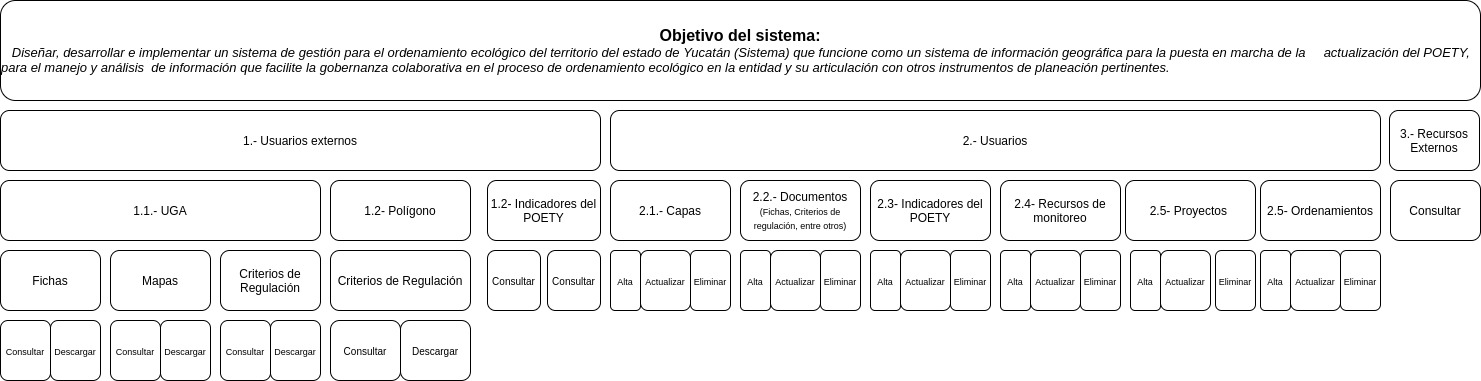
\includegraphics[width=1\textwidth, height=.5\textwidth]{images/PrioritizationRequirements}
\end{figure}
\useportrait

\restoregeometry

\uselandscape
\subsection{Diagrama de Casos de Uso}

\begin{figure}[h]

\centering
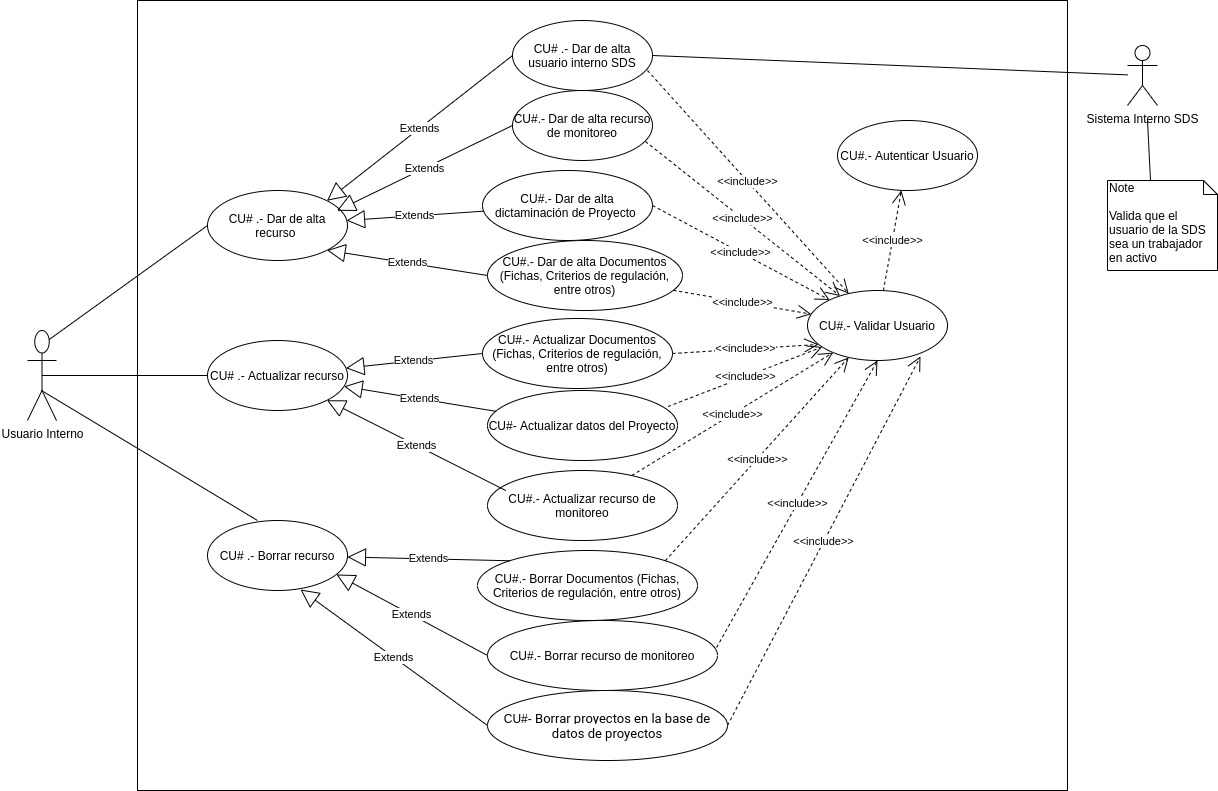
\includegraphics[width=1\textwidth, height=.39\textwidth]{images/AdminiInsumos}
\caption{Diagrama de Administración de Recursos}\label{fig:consumorec_cu_diag}

\end{figure}
\useportrait

\uselandscape

\begin{figure}[h]

\centering
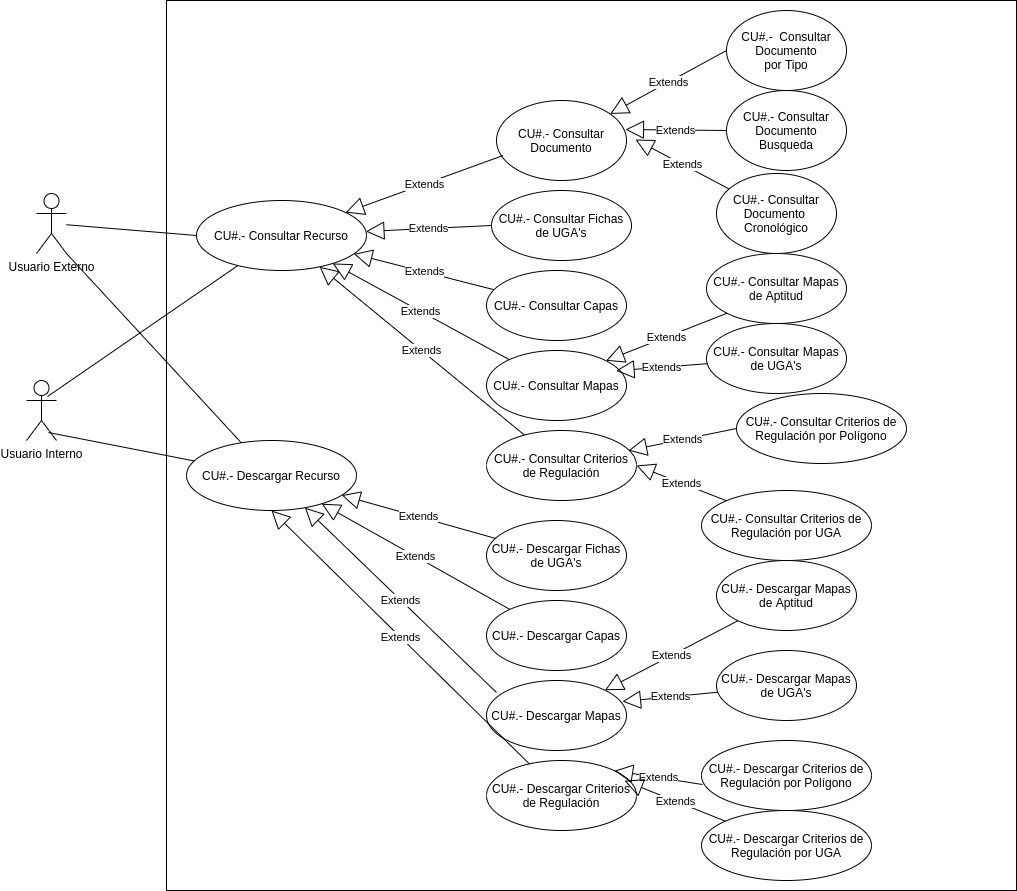
\includegraphics[width=1\textwidth, height=.43\textwidth]{images/ConsumoRecursosPropuesta}
\caption{Diagrama de Consumo de Recursos}\label{fig:consumorec_cu_diag_prop}

\end{figure}
\useportrait
\restoregeometry



\subsection{Descripción de Módulos y Casos de Uso}


\begin{longtable}{@{\extracolsep{6pt}}l p{7.5cm}}
\caption{Módulos y Casos de Uso}\label{item:mod_cu}\\
\\[-1.8ex]\hline
\endhead
\hline \\[-1.8ex]
 \multicolumn{1}{c} {\textit{\textbf{Módulo}}} & {\textit{\textbf{Casos de Uso}}} \\
\hline \\[-1ex]

& Consultar fichas de UGAs\\
\cline{2-2}
 & Descargar ficha de UGA\\
\cline{2-2}
 & Consultar capas de insumo para el ordenamiento\\
\cline{2-2}
 & Consultar mapas de aptitud\\
\cline{2-2}
 & Descargar capas\\
\cline{2-2}
 & Consultar mapas de UGAs\\
\cline{2-2}
& Consultar documentos relacionados con la formulación del (POETY, POETCY, o POEL)\\
\cline{2-2}
Consultas y descargas & Consultar documentos del (POETY, POETCY, o POEL) por búsqueda\\
\cline{2-2}
 & Consultar documentos del (POETY, POETCY, o POEL) por orden cronológico\\
\cline{2-2}
 & Consultar documentos del (POETY, POETCY, o POEL) por tipo\\
\cline{2-2}
 & Descargar documento\\
\cline{2-2}
 & Consultar criterios de regulación por polígono\\
\cline{2-2}
 & Descargar criterios de regulación por polígono\\
\cline{2-2}
 & Descargar criterios de regulación por UGA\\
\cline{2-2}
 & Consultar indicadores del (POETY, POETCY, o POEL) \\
\hline
\cline{2-2}
 & Dar de alta documentos (fichas, u otros)\\
\cline{2-2}
 & Dar de alta capas \\
\cline{2-2}
 & Actualizar documentos (fichas, u otros)\\
\cline{2-2}
& Actualizar capas \\
\cline{2-2}
Actualización de recursos & Borrar documentos (fichas, u otros)\\
\cline{2-2}
 & Borrar capas \\
\cline{2-2}
 & Dar de alta recursos de monitoreo \\
\cline{2-2}
 & Actualizar recursos de monitoreo \\
\cline{2-2}
 & Borrar recursos de monitoreo\\
\hline
 &
Obtener un informe sobre los criterios de regulación y los impactos acumulados\\
\cline{2-2}
Automatización de reportes & Dar de alta dictamen de un proyecto\\
\cline{2-2}
  & Modificar los datos de un proyecto \\
\cline{2-2}
 & Borrar proyectos en la base de datos de proyectos\\
\hline
 & Dar de alta usuario interno de SDS \\
\cline{2-2}
 & Dar de baja usuario interno de SDS  \\
\cline{2-2}
 & Modificar datos de usuarios internos de SDS\\
\cline{2-2}
Módulo de administración & Validar usuraio \\
\cline{2-2}
 & Autenticar usuario\\
\cline{2-2}
 & Dar de alta un ordenamiento\\
\cline{2-2}
 & Borrar un ordenamiento\\
\cline{2-2}
 & Modificar datos generales de un ordenamiento\\
\hline
\hline \\[-1.8ex]
  \\
\end{longtable}

\pagebreak
\subsection{Casos de Uso}




%%%%%%%%%%%%%%%%%%%%%%%%%%%%%%%%%%%%%%%%%%%%%%%%%%%%%%%%%%
%%%%%% CU: Consultar fichas de UGAs
%%%%%%%%%%%%%%%%%%%%%%%%%%%%%%%%%%%%%%%%%%%%%%%%%%%%%%%%%%



\begin{longtable}{@{\extracolsep{8pt}}l p{8.5cm}}
\caption{Caso de uso: Consultar fichas de UGAs }\label{item: consultar_fichas_de_ugas }\\
\\[-1.8ex]\hline
\endhead
\hline \\[-1.8ex]
 \multicolumn{1}{c} {\textit{\textbf{CASO DE USO}}}& {\textit{\textbf{ Consultar fichas de UGAs }}} \\
\hline \\[-1ex]
ID. DEL CU&  0 \\
\hline\\[-1ex]
ACTORES PARTICIPANTES & 
\par - Usuario externo

\par - Usuario interno

\\
\hline \\[-1ex]
BREVE DESCRIPCIÓN & El usuario selecciona la UGA en el mapa, solicita la ficha de esa UGA y el sistema despliega la visualización de la ficha \\
\hline \\[-1ex]

PRE-CONDICIONES & \textbf{Del proceso}: \par\vspace{.1cm} Ninguna, puede ocurrir en cualquier momento
 \par\vspace{.2cm} \textbf{Del sistema} \par\vspace{.1cm} La ficha de la UGA está disponible \\
\hline \\[-1ex]

FLUJO PRINCIPAL &

 1. El usuario accede a la bitácora del ordenamientos \par\vspace{.1cm}

 2. El usuario selcciona el ordenamiento deseado (POETY, POETCY, o POEL) \par\vspace{.1cm}

 3. El usuario seleciona la capa de UGAs \par\vspace{.1cm}

 4. El usuario selecciona la UGA de interés \par\vspace{.1cm}

 5. El usuario solicita la ficha de la UGA de interés \par\vspace{.1cm}

 6. El usuario descarga la ficha(A1)  \par\vspace{.1cm}

\\
\hline \\[-1ex]

FLUJOS ALTERNOS & 
\par (A1) El usuario solicita la descarga de la ficha (CU1)

\par (A2) El usuario solicita la descarga de los criterios de regulación por UGA (CU13)



\\
\hline \\[-1ex]

FLUJOS DE EXCEPCIÓN & 
\par\vspace{.1cm} (E1) En caso de no existir la ficha de la UGA solicitada, levantar un reporte


\\%%%<---- Este salto de linea faltaba

\hline \\[-1ex]
POST-CONDICIONES & 
\\
\hline
\hline \\[-1.8ex]
 \\
\end{longtable}


\pagebreak


%%%%%%%%%%%%%%%%%%%%%%%%%%%%%%%%%%%%%%%%%%%%%%%%%%%%%%%%%%
%%%%%% CU: Descargar ficha de UGA
%%%%%%%%%%%%%%%%%%%%%%%%%%%%%%%%%%%%%%%%%%%%%%%%%%%%%%%%%%



\begin{longtable}{@{\extracolsep{8pt}}l p{8.5cm}}
\caption{Caso de uso: Descargar ficha de UGA }\label{item: descargar_ficha_de_uga }\\
\\[-1.8ex]\hline
\endhead
\hline \\[-1.8ex]
 \multicolumn{1}{c} {\textit{\textbf{CASO DE USO}}}& {\textit{\textbf{ Descargar ficha de UGA }}} \\
\hline \\[-1ex]
ID. DEL CU&  1 \\
\hline\\[-1ex]
ACTORES PARTICIPANTES & 
\par - Usuario externo

\par - Usuario interno

\\
\hline \\[-1ex]
BREVE DESCRIPCIÓN & El usuario descarga la ficha técnica de una unidad de gestión ambiental  \\
\hline \\[-1ex]

PRE-CONDICIONES & \textbf{Del proceso}: \par\vspace{.1cm} El usuario realiza la consulta de una UGA para visualizar su ficha
 \par\vspace{.2cm} \textbf{Del sistema} \par\vspace{.1cm} La ficha de la UGA está disponible \\
\hline \\[-1ex]

FLUJO PRINCIPAL &

 1. El usuario accede a la bitácora del ordenamientos \par\vspace{.1cm}

 2. El usuario selcciona el ordenamiento deseado (POETY, POETCY, o POEL) \par\vspace{.1cm}

 3. El usuario la capa de UGAs \par\vspace{.1cm}

 4. El usuario solicita la ficha de la UGA de interés \par\vspace{.1cm}

 5. El usuario descarga la ficha \par\vspace{.1cm}

\\
\hline \\[-1ex]

FLUJOS ALTERNOS & 


\\
\hline \\[-1ex]

FLUJOS DE EXCEPCIÓN & 
\par\vspace{.1cm} (E1) En caso de no existir la ficha de la UGA solicitada, levantar un reporte


\\%%%<---- Este salto de linea faltaba

\hline \\[-1ex]
POST-CONDICIONES & 
\\
\hline
\hline \\[-1.8ex]
 \\
\end{longtable}


\pagebreak


%%%%%%%%%%%%%%%%%%%%%%%%%%%%%%%%%%%%%%%%%%%%%%%%%%%%%%%%%%
%%%%%% CU: Consultar capas de insumo para el ordenamiento
%%%%%%%%%%%%%%%%%%%%%%%%%%%%%%%%%%%%%%%%%%%%%%%%%%%%%%%%%%



\begin{longtable}{@{\extracolsep{8pt}}l p{8.5cm}}
\caption{Caso de uso: Consultar capas de insumo para el ordenamiento }\label{item: consultar_capas_de_insumo_para_el_ordenamiento }\\
\\[-1.8ex]\hline
\endhead
\hline \\[-1.8ex]
 \multicolumn{1}{c} {\textit{\textbf{CASO DE USO}}}& {\textit{\textbf{ Consultar capas de insumo para el ordenamiento }}} \\
\hline \\[-1ex]
ID. DEL CU&  2 \\
\hline\\[-1ex]
ACTORES PARTICIPANTES & 
\par - Usuario externo

\par - Usuario interno

\\
\hline \\[-1ex]
BREVE DESCRIPCIÓN & El usuario consulta las capas de insumo que conforman el mapa de aptitud de un sector específico  \\
\hline \\[-1ex]

PRE-CONDICIONES & \textbf{Del proceso}: \par\vspace{.1cm} El usuario selecciona un sector
 \par\vspace{.2cm} \textbf{Del sistema} \par\vspace{.1cm} Las capas de los insumos están disponibles y tienen un estilo asociado \\
\hline \\[-1ex]

FLUJO PRINCIPAL &

 1. El usuario accede a la bitácora del ordenamientos \par\vspace{.1cm}

 2. El usuario selcciona el ordenamiento deseado (POETY, POETCY, o POEL) \par\vspace{.1cm}

 3. El usuario selcciona la sección de diagnóstico \par\vspace{.1cm}

 4. El sistema muestra una lista de sectores  \par\vspace{.1cm}

 5. El usuario elige el sector de interés \par\vspace{.1cm}

 6. El sistema visualiza el mapa de aptitud del sector (CU3) \par\vspace{.1cm}

 7. El usuario selecciona la capa de insumo deseada \par\vspace{.1cm}

 8. El sistema muestra la capa deseada y la función de valor asociada \par\vspace{.1cm}

\\
\hline \\[-1ex]

FLUJOS ALTERNOS & 
\par (A1) El usuario descarga la capa de insumo (CU4)



\\
\hline \\[-1ex]

FLUJOS DE EXCEPCIÓN & 
\par\vspace{.1cm} (E1) En caso de no existir la capa de insumo solicitada, levantar un reporte


\\%%%<---- Este salto de linea faltaba

\hline \\[-1ex]
POST-CONDICIONES & 
\\
\hline
\hline \\[-1.8ex]
 \\
\end{longtable}


\pagebreak


%%%%%%%%%%%%%%%%%%%%%%%%%%%%%%%%%%%%%%%%%%%%%%%%%%%%%%%%%%
%%%%%% CU: Consultar mapas de aptitud
%%%%%%%%%%%%%%%%%%%%%%%%%%%%%%%%%%%%%%%%%%%%%%%%%%%%%%%%%%



\begin{longtable}{@{\extracolsep{8pt}}l p{8.5cm}}
\caption{Caso de uso: Consultar mapas de aptitud }\label{item: consultar_mapas_de_aptitud }\\
\\[-1.8ex]\hline
\endhead
\hline \\[-1.8ex]
 \multicolumn{1}{c} {\textit{\textbf{CASO DE USO}}}& {\textit{\textbf{ Consultar mapas de aptitud }}} \\
\hline \\[-1ex]
ID. DEL CU&  3 \\
\hline\\[-1ex]
ACTORES PARTICIPANTES & 
\par - Usuario externo

\par - Usuario interno

\\
\hline \\[-1ex]
BREVE DESCRIPCIÓN & El usuario visualiza el mapa de aptitud por sector  \\
\hline \\[-1ex]

PRE-CONDICIONES & \textbf{Del proceso}: \par\vspace{.1cm} Ninguna, puede ocurrir en cualquier momento
 \par\vspace{.2cm} \textbf{Del sistema} \par\vspace{.1cm} La capa está disponible \\
\hline \\[-1ex]

FLUJO PRINCIPAL &

 1. El usuario accede a la bitácora del ordenamientos \par\vspace{.1cm}

 2. El usuario selcciona el ordenamiento deseado (POETY, POETCY, o POEL) \par\vspace{.1cm}

 3. El usuario selcciona la sección de diagnóstico \par\vspace{.1cm}

 4. El sistema muestra una lista de sectores  \par\vspace{.1cm}

 5. El usuario elige el sector de interés \par\vspace{.1cm}

 6. El sistema visualiza el mapa de aptitud del sector y despliega una lista de los insumos \par\vspace{.1cm}

\\
\hline \\[-1ex]

FLUJOS ALTERNOS & 
\par (A1) El usuario visualiza las capas de insumo (CU2)



\\
\hline \\[-1ex]

FLUJOS DE EXCEPCIÓN & 
\par\vspace{.1cm} (E1) En caso de no visualizar el mapa, levantar un reporte


\\%%%<---- Este salto de linea faltaba

\hline \\[-1ex]
POST-CONDICIONES & 
\\
\hline
\hline \\[-1.8ex]
 \\
\end{longtable}


\pagebreak


%%%%%%%%%%%%%%%%%%%%%%%%%%%%%%%%%%%%%%%%%%%%%%%%%%%%%%%%%%
%%%%%% CU: Descargar capas
%%%%%%%%%%%%%%%%%%%%%%%%%%%%%%%%%%%%%%%%%%%%%%%%%%%%%%%%%%



\begin{longtable}{@{\extracolsep{8pt}}l p{8.5cm}}
\caption{Caso de uso: Descargar capas }\label{item: descargar_capas }\\
\\[-1.8ex]\hline
\endhead
\hline \\[-1.8ex]
 \multicolumn{1}{c} {\textit{\textbf{CASO DE USO}}}& {\textit{\textbf{ Descargar capas }}} \\
\hline \\[-1ex]
ID. DEL CU&  4 \\
\hline\\[-1ex]
ACTORES PARTICIPANTES & 
\par - Usuario externo

\par - Usuario interno

\\
\hline \\[-1ex]
BREVE DESCRIPCIÓN & El usuario descarga la capa visualizada  \\
\hline \\[-1ex]

PRE-CONDICIONES & \textbf{Del proceso}: \par\vspace{.1cm} La capa esta visualizada en el sistema
 \par\vspace{.2cm} \textbf{Del sistema} \par\vspace{.1cm} La capa está disponible \\
\hline \\[-1ex]

FLUJO PRINCIPAL &

 1. El usuario accede a la bitácora del ordenamientos \par\vspace{.1cm}

 2. El usuario selcciona el ordenamiento deseado (POETY, POETCY, o POEL) \par\vspace{.1cm}

 3. El usuario selcciona la sección de diagnóstico \par\vspace{.1cm}

 4. El usuario visualiza una capa mediante los casos de uso (CU2,CU3,CU5) \par\vspace{.1cm}

 5. El usuario solicita la descarga \par\vspace{.1cm}

 6. El sistema incluye en la descarga la capa geográfica y los metadatos asociados \par\vspace{.1cm}

\\
\hline \\[-1ex]

FLUJOS ALTERNOS & 
\par NA 



\\
\hline \\[-1ex]

FLUJOS DE EXCEPCIÓN & 
\par\vspace{.1cm} (E1) En caso de no descargarse la capa  solicitada, levantar un reporte


\\%%%<---- Este salto de linea faltaba

\hline \\[-1ex]
POST-CONDICIONES & 
\\
\hline
\hline \\[-1.8ex]
 \\
\end{longtable}


\pagebreak


%%%%%%%%%%%%%%%%%%%%%%%%%%%%%%%%%%%%%%%%%%%%%%%%%%%%%%%%%%
%%%%%% CU: Consultar mapas de UGAs
%%%%%%%%%%%%%%%%%%%%%%%%%%%%%%%%%%%%%%%%%%%%%%%%%%%%%%%%%%



\begin{longtable}{@{\extracolsep{8pt}}l p{8.5cm}}
\caption{Caso de uso: Consultar mapas de UGAs }\label{item: consultar_mapas_de_ugas }\\
\\[-1.8ex]\hline
\endhead
\hline \\[-1.8ex]
 \multicolumn{1}{c} {\textit{\textbf{CASO DE USO}}}& {\textit{\textbf{ Consultar mapas de UGAs }}} \\
\hline \\[-1ex]
ID. DEL CU&  5 \\
\hline\\[-1ex]
ACTORES PARTICIPANTES & 
\par - Usuario externo

\par - Usuario interno

\\
\hline \\[-1ex]
BREVE DESCRIPCIÓN & El usuario visualiza las unidades de gestión ambiental \\
\hline \\[-1ex]

PRE-CONDICIONES & \textbf{Del proceso}: \par\vspace{.1cm} Ninguna, puede ocurrir en cualquier momento
 \par\vspace{.2cm} \textbf{Del sistema} \par\vspace{.1cm} La ficha de la UGA está disponible \\
\hline \\[-1ex]

FLUJO PRINCIPAL &

 1. El usuario accede a la bitácora del ordenamientos \par\vspace{.1cm}

 2. El usuario selcciona el ordenamiento deseado (POETY, POETCY, o POEL) \par\vspace{.1cm}

 3. El usuario la capa de UGAs \par\vspace{.1cm}

 4. El sistema muestra la capa de UGAs  \par\vspace{.1cm}

\\
\hline \\[-1ex]

FLUJOS ALTERNOS & 
\par (A1) El usuario solicita la descarga de la capa de las ugas (CU4)



\\
\hline \\[-1ex]

FLUJOS DE EXCEPCIÓN & 
\par\vspace{.1cm} (E1) En caso de no visualizar el mapa solicitado, levantar un reporte


\\%%%<---- Este salto de linea faltaba

\hline \\[-1ex]
POST-CONDICIONES & 
\\
\hline
\hline \\[-1.8ex]
 \\
\end{longtable}


\pagebreak


%%%%%%%%%%%%%%%%%%%%%%%%%%%%%%%%%%%%%%%%%%%%%%%%%%%%%%%%%%
%%%%%% CU: Consultar documento relacionado con la formulación del (POETY, POETCY, o POEL)
%%%%%%%%%%%%%%%%%%%%%%%%%%%%%%%%%%%%%%%%%%%%%%%%%%%%%%%%%%



\begin{longtable}{@{\extracolsep{8pt}}l p{8.5cm}}
\caption{Caso de uso: Consultar documento relacionado con la formulación del (POETY, POETCY, o POEL) }\label{item: consultar_documento_relacionado_con_la_formulacion_del_poety_poetcy_o_poel }\\
\\[-1.8ex]\hline
\endhead
\hline \\[-1.8ex]
 \multicolumn{1}{c} {\textit{\textbf{CASO DE USO}}}& {\textit{\textbf{ Consultar documento relacionado con la formulación del (POETY, POETCY, o POEL) }}} \\
\hline \\[-1ex]
ID. DEL CU&  6 \\
\hline\\[-1ex]
ACTORES PARTICIPANTES & 
\par - Usuario externo

\par - Usuario interno

\\
\hline \\[-1ex]
BREVE DESCRIPCIÓN & El usuario consulta cualquier documento relacionado con la formulación del POETY (por búsqueda, por orden cronológico, por categoría) \\
\hline \\[-1ex]

PRE-CONDICIONES & \textbf{Del proceso}: \par\vspace{.1cm} Ninguna, puede ocurrir en cualquier momento.
 \par\vspace{.2cm} \textbf{Del sistema} \par\vspace{.1cm} El documento este disponible \\
\hline \\[-1ex]

FLUJO PRINCIPAL &

 1. El usuario accede a la bitácora del ordenamientos \par\vspace{.1cm}

 2. El usuario selcciona el ordenamiento deseado (POETY, POETCY, o POEL) \par\vspace{.1cm}

 3. El usuario selecciona la sección de documentos de la formulación del ordenamiento específico  \par\vspace{.1cm}

 4. El sistema despliega los modos de búsqueda (por búsqueda de palabra clave,por orden cronológico, por tipo) Ver casos de uso (CU7, CU8, CU9) \par\vspace{.1cm}

\\
\hline \\[-1ex]

FLUJOS ALTERNOS & 
\par NA



\\
\hline \\[-1ex]

FLUJOS DE EXCEPCIÓN & 
\par\vspace{.1cm} NA


\\%%%<---- Este salto de linea faltaba

\hline \\[-1ex]
POST-CONDICIONES & 
\\
\hline
\hline \\[-1.8ex]
 \\
\end{longtable}


\pagebreak


%%%%%%%%%%%%%%%%%%%%%%%%%%%%%%%%%%%%%%%%%%%%%%%%%%%%%%%%%%
%%%%%% CU: Consultar documento del (POETY, POETCY, o POEL) por búsqueda
%%%%%%%%%%%%%%%%%%%%%%%%%%%%%%%%%%%%%%%%%%%%%%%%%%%%%%%%%%



\begin{longtable}{@{\extracolsep{8pt}}l p{8.5cm}}
\caption{Caso de uso: Consultar documento del (POETY, POETCY, o POEL) por búsqueda }\label{item: consultar_documento_del_poety_poetcy_o_poel_por_busqueda }\\
\\[-1.8ex]\hline
\endhead
\hline \\[-1.8ex]
 \multicolumn{1}{c} {\textit{\textbf{CASO DE USO}}}& {\textit{\textbf{ Consultar documento del (POETY, POETCY, o POEL) por búsqueda }}} \\
\hline \\[-1ex]
ID. DEL CU&  7 \\
\hline\\[-1ex]
ACTORES PARTICIPANTES & 
\par - Usuario externo

\par - Usuario interno

\\
\hline \\[-1ex]
BREVE DESCRIPCIÓN & El usuario consulta un documento relacionado con la formulación del POETY por búsqueda de palabra(s) clave(s) \\
\hline \\[-1ex]

PRE-CONDICIONES & \textbf{Del proceso}: \par\vspace{.1cm} El usuario elige el modo de búsqueda por palabra clave (CU6)
 \par\vspace{.2cm} \textbf{Del sistema} \par\vspace{.1cm} El documento este disponible \\
\hline \\[-1ex]

FLUJO PRINCIPAL &

 1. El usuario accede a la bitácora del ordenamientos \par\vspace{.1cm}

 2. El usuario selcciona el ordenamiento deseado (POETY, POETCY, o POEL) \par\vspace{.1cm}

 3. El usuario selecciona la sección de documentos de la formulación del ordenamiento específico  \par\vspace{.1cm}

 4. El usuario selecciona el modo de  búsqueda de palabra clave \par\vspace{.1cm}

 5. El usuario ingresa la palabra(s) clave relacionada(s) con el documento \par\vspace{.1cm}

 6. El sistema despliega una lista de documentos relacionados \par\vspace{.1cm}

 7. El usuario selecciona el documento deseado \par\vspace{.1cm}

 8. El sistema ejecuta la visualización del documento seleccionado \par\vspace{.1cm}

\\
\hline \\[-1ex]

FLUJOS ALTERNOS & 
\par (A1) El usuario solicita la descarga del documento (CU10)



\\
\hline \\[-1ex]

FLUJOS DE EXCEPCIÓN & 
\par\vspace{.1cm} NA


\\%%%<---- Este salto de linea faltaba

\hline \\[-1ex]
POST-CONDICIONES & 
\\
\hline
\hline \\[-1.8ex]
 \\
\end{longtable}


\pagebreak


%%%%%%%%%%%%%%%%%%%%%%%%%%%%%%%%%%%%%%%%%%%%%%%%%%%%%%%%%%
%%%%%% CU: Consultar documento del (POETY, POETCY, o POEL) por orden cronológico
%%%%%%%%%%%%%%%%%%%%%%%%%%%%%%%%%%%%%%%%%%%%%%%%%%%%%%%%%%



\begin{longtable}{@{\extracolsep{8pt}}l p{8.5cm}}
\caption{Caso de uso: Consultar documento del (POETY, POETCY, o POEL) por orden cronológico }\label{item: consultar_documento_del_poety_poetcy_o_poel_por_orden_cronologico }\\
\\[-1.8ex]\hline
\endhead
\hline \\[-1.8ex]
 \multicolumn{1}{c} {\textit{\textbf{CASO DE USO}}}& {\textit{\textbf{ Consultar documento del (POETY, POETCY, o POEL) por orden cronológico }}} \\
\hline \\[-1ex]
ID. DEL CU&  8 \\
\hline\\[-1ex]
ACTORES PARTICIPANTES & 
\par - Usuario externo

\par - Usuario interno

\\
\hline \\[-1ex]
BREVE DESCRIPCIÓN & El usuario consulta un documento relacionado con la formulación del POETY por orden cronológico \\
\hline \\[-1ex]

PRE-CONDICIONES & \textbf{Del proceso}: \par\vspace{.1cm} Ninguna, puede ocurrir en cualquier momento.
 \par\vspace{.2cm} \textbf{Del sistema} \par\vspace{.1cm} El documento este disponible \\
\hline \\[-1ex]

FLUJO PRINCIPAL &

 1. El usuario accede a la bitácora del ordenamientos \par\vspace{.1cm}

 2. El usuario selcciona el ordenamiento deseado (POETY, POETCY, o POEL) \par\vspace{.1cm}

 3. El usuario selecciona la sección de documentos de la formulación del ordenamiento específico  \par\vspace{.1cm}

 4. El usuario selecciona el modo de  búsqueda por orden cronológico \par\vspace{.1cm}

 5. El sistema despliega una lista de documentos por orden cronológico \par\vspace{.1cm}

 6. El usuario selecciona el documento deseado \par\vspace{.1cm}

 7. El sistema ejecuta la visualización del documento seleccionado \par\vspace{.1cm}

\\
\hline \\[-1ex]

FLUJOS ALTERNOS & 
\par (A1) El usuario solicita la descarga del documento (CU10)



\\
\hline \\[-1ex]

FLUJOS DE EXCEPCIÓN & 
\par\vspace{.1cm} NA


\\%%%<---- Este salto de linea faltaba

\hline \\[-1ex]
POST-CONDICIONES & 
\\
\hline
\hline \\[-1.8ex]
 \\
\end{longtable}


\pagebreak


%%%%%%%%%%%%%%%%%%%%%%%%%%%%%%%%%%%%%%%%%%%%%%%%%%%%%%%%%%
%%%%%% CU: Consultar documento del (POETY, POETCY, o POEL) por tipo
%%%%%%%%%%%%%%%%%%%%%%%%%%%%%%%%%%%%%%%%%%%%%%%%%%%%%%%%%%



\begin{longtable}{@{\extracolsep{8pt}}l p{8.5cm}}
\caption{Caso de uso: Consultar documento del (POETY, POETCY, o POEL) por tipo }\label{item: consultar_documento_del_poety_poetcy_o_poel_por_tipo }\\
\\[-1.8ex]\hline
\endhead
\hline \\[-1.8ex]
 \multicolumn{1}{c} {\textit{\textbf{CASO DE USO}}}& {\textit{\textbf{ Consultar documento del (POETY, POETCY, o POEL) por tipo }}} \\
\hline \\[-1ex]
ID. DEL CU&  9 \\
\hline\\[-1ex]
ACTORES PARTICIPANTES & 
\par - Usuario externo

\par - Usuario interno

\\
\hline \\[-1ex]
BREVE DESCRIPCIÓN & El usuario consulta un documento relacionado con la formulación del POETY por tipo \\
\hline \\[-1ex]

PRE-CONDICIONES & \textbf{Del proceso}: \par\vspace{.1cm} Ninguna, puede ocurrir en cualquier momento.
 \par\vspace{.2cm} \textbf{Del sistema} \par\vspace{.1cm} El documento este disponible \\
\hline \\[-1ex]

FLUJO PRINCIPAL &

 1. El usuario accede a la bitácora del ordenamientos \par\vspace{.1cm}

 2. El usuario selcciona el ordenamiento deseado (POETY, POETCY, o POEL) \par\vspace{.1cm}

 3. El usuario selecciona la sección de documentos de la formulación del ordenamiento específico  \par\vspace{.1cm}

 4. El usuario selecciona el modo de  búsqueda por tipo \par\vspace{.1cm}

 5. El sistema despliega una lista de documentos por tipo de documento \par\vspace{.1cm}

 6. El usuario selecciona el tipo de docuemento  \par\vspace{.1cm}

 7. El sistema despliega una lista de los documentos en la categoria seleccionada \par\vspace{.1cm}

 8. El usuario selecciona el documento deseado \par\vspace{.1cm}

 9. El sistema ejecuta la visualización del documento deseado \par\vspace{.1cm}

\\
\hline \\[-1ex]

FLUJOS ALTERNOS & 
\par (A1) El usuario solicita la descarga del documento (CU10)



\\
\hline \\[-1ex]

FLUJOS DE EXCEPCIÓN & 
\par\vspace{.1cm} NA


\\%%%<---- Este salto de linea faltaba

\hline \\[-1ex]
POST-CONDICIONES & 
\\
\hline
\hline \\[-1.8ex]
 \\
\end{longtable}


\pagebreak


%%%%%%%%%%%%%%%%%%%%%%%%%%%%%%%%%%%%%%%%%%%%%%%%%%%%%%%%%%
%%%%%% CU: Descargar documento
%%%%%%%%%%%%%%%%%%%%%%%%%%%%%%%%%%%%%%%%%%%%%%%%%%%%%%%%%%



\begin{longtable}{@{\extracolsep{8pt}}l p{8.5cm}}
\caption{Caso de uso: Descargar documento }\label{item: descargar_documento }\\
\\[-1.8ex]\hline
\endhead
\hline \\[-1.8ex]
 \multicolumn{1}{c} {\textit{\textbf{CASO DE USO}}}& {\textit{\textbf{ Descargar documento }}} \\
\hline \\[-1ex]
ID. DEL CU&  10 \\
\hline\\[-1ex]
ACTORES PARTICIPANTES & 
\par - Usuario externo

\par - Usuario interno

\\
\hline \\[-1ex]
BREVE DESCRIPCIÓN & EL usuario descarga el documento relacionado con la formulación del POETY \\
\hline \\[-1ex]

PRE-CONDICIONES & \textbf{Del proceso}: \par\vspace{.1cm} Ninguna, puede ocurrir en cualquier momento.
 \par\vspace{.2cm} \textbf{Del sistema} \par\vspace{.1cm} El documento este disponible \\
\hline \\[-1ex]

FLUJO PRINCIPAL &

 1. El usuario accede a la bitácora del ordenamientos \par\vspace{.1cm}

 2. El usuario selcciona el ordenamiento deseado (POETY, POETCY, o POEL) \par\vspace{.1cm}

 3. El usuario selecciona la sección de documentos de la formulación del ordenamiento específico  \par\vspace{.1cm}

 4. El usuario selecciona el modo de  búsqueda  \par\vspace{.1cm}

 5. El sistema despliega una lista de documentos según el tipo de búsqueda (CU6) \par\vspace{.1cm}

 6. El sistema despliega una lista de los documentos \par\vspace{.1cm}

 7. El usuario selecciona el documento deseado \par\vspace{.1cm}

 8. El sistema ejecuta la visualización del documento deseado \par\vspace{.1cm}

 9. El usuario solicita la descarga del documento \par\vspace{.1cm}

\\
\hline \\[-1ex]

FLUJOS ALTERNOS & 
\par NA



\\
\hline \\[-1ex]

FLUJOS DE EXCEPCIÓN & 
\par\vspace{.1cm} NA


\\%%%<---- Este salto de linea faltaba

\hline \\[-1ex]
POST-CONDICIONES & 
\\
\hline
\hline \\[-1.8ex]
 \\
\end{longtable}


\pagebreak


%%%%%%%%%%%%%%%%%%%%%%%%%%%%%%%%%%%%%%%%%%%%%%%%%%%%%%%%%%
%%%%%% CU: Consultar criterios de regulación por polígono
%%%%%%%%%%%%%%%%%%%%%%%%%%%%%%%%%%%%%%%%%%%%%%%%%%%%%%%%%%



\begin{longtable}{@{\extracolsep{8pt}}l p{8.5cm}}
\caption{Caso de uso: Consultar criterios de regulación por polígono }\label{item: consultar_criterios_de_regulacion_por_poligono }\\
\\[-1.8ex]\hline
\endhead
\hline \\[-1.8ex]
 \multicolumn{1}{c} {\textit{\textbf{CASO DE USO}}}& {\textit{\textbf{ Consultar criterios de regulación por polígono }}} \\
\hline \\[-1ex]
ID. DEL CU&  11 \\
\hline\\[-1ex]
ACTORES PARTICIPANTES & 
\par - Usuario externo

\par - Usuario interno

\\
\hline \\[-1ex]
BREVE DESCRIPCIÓN & El usuario consulta los criterios de regulación que aplican en un área de interés \\
\hline \\[-1ex]

PRE-CONDICIONES & \textbf{Del proceso}: \par\vspace{.1cm} Ninguna, puede ocurrir en cualquier momento
 \par\vspace{.2cm} \textbf{Del sistema} \par\vspace{.1cm} Ninguna \\
\hline \\[-1ex]

FLUJO PRINCIPAL &

 1. El usuario accede a la bitácora del ordenamiento \par\vspace{.1cm}

 2. El usuario selecciona la sección de criterios de regulación \par\vspace{.1cm}

 3. El usuario provee un poligono de interés en formato shapefile \par\vspace{.1cm}

 4. El sistema despliega un mapa con la intersección del polígono proporcionado y las UGAS estatales y/o locales y una lista de los criterios de regulación que aplican para cada una de las interesecciones \par\vspace{.1cm}

\\
\hline \\[-1ex]

FLUJOS ALTERNOS & 
\par (A1) El usuario solicita la descarga de los criterios de regulación (CU12)



\\
\hline \\[-1ex]

FLUJOS DE EXCEPCIÓN & 
\par\vspace{.1cm} (E1) En caso de que el shapefile proporcionado sea defectuoso el sistema muestra un mensaje "capa no válida" y regresa a la sección de criterios de regulación 

\par\vspace{.1cm} (E2) En caso de no aplicar ningún criterio de regulación, el sistema responde que no aplica ningún criterio y regresa a la sección de criterios de regulación


\\%%%<---- Este salto de linea faltaba

\hline \\[-1ex]
POST-CONDICIONES & 
\\
\hline
\hline \\[-1.8ex]
 \\
\end{longtable}


\pagebreak


%%%%%%%%%%%%%%%%%%%%%%%%%%%%%%%%%%%%%%%%%%%%%%%%%%%%%%%%%%
%%%%%% CU: Descargar criterios de regulación por polígono
%%%%%%%%%%%%%%%%%%%%%%%%%%%%%%%%%%%%%%%%%%%%%%%%%%%%%%%%%%



\begin{longtable}{@{\extracolsep{8pt}}l p{8.5cm}}
\caption{Caso de uso: Descargar criterios de regulación por polígono }\label{item: descargar_criterios_de_regulacion_por_poligono }\\
\\[-1.8ex]\hline
\endhead
\hline \\[-1.8ex]
 \multicolumn{1}{c} {\textit{\textbf{CASO DE USO}}}& {\textit{\textbf{ Descargar criterios de regulación por polígono }}} \\
\hline \\[-1ex]
ID. DEL CU&  12 \\
\hline\\[-1ex]
ACTORES PARTICIPANTES & 
\par - Usuario externo

\par - Usuario interno

\\
\hline \\[-1ex]
BREVE DESCRIPCIÓN & El usuario descarga los criterios de regulación que aplican en un polígono específico \\
\hline \\[-1ex]

PRE-CONDICIONES & \textbf{Del proceso}: \par\vspace{.1cm} El usuario realiza la consulta de criterios de regulación por polígono (CU11)
 \par\vspace{.2cm} \textbf{Del sistema} \par\vspace{.1cm} Ninguna \\
\hline \\[-1ex]

FLUJO PRINCIPAL &

 1. El usuario accede a la bitácora del ordenamiento \par\vspace{.1cm}

 2. El usuario selecciona la sección de criterios de regulación \par\vspace{.1cm}

 3. El usuario provee un poligono de interés en formato shapefile \par\vspace{.1cm}

 4. El sistema despliega un mapa con la intersección del polígono proporcionado y las UGAS estatales y/o locales y una lista de los criterios de regulación que aplican para cada una de las interesecciones \par\vspace{.1cm}

 5. El usuario descarga un documento que incluye el mapa y la lista de los criterios de regulación o solo la lista de criterios de regulación en formato csv o xls \par\vspace{.1cm}

\\
\hline \\[-1ex]

FLUJOS ALTERNOS & 
\par NA



\\
\hline \\[-1ex]

FLUJOS DE EXCEPCIÓN & 
\par\vspace{.1cm} (E1) En caso de error al  descargar la lista solicitada, levantar un reporte


\\%%%<---- Este salto de linea faltaba

\hline \\[-1ex]
POST-CONDICIONES & 
\\
\hline
\hline \\[-1.8ex]
 \\
\end{longtable}


\pagebreak


%%%%%%%%%%%%%%%%%%%%%%%%%%%%%%%%%%%%%%%%%%%%%%%%%%%%%%%%%%
%%%%%% CU: Descargar criterios de regulación por UGA
%%%%%%%%%%%%%%%%%%%%%%%%%%%%%%%%%%%%%%%%%%%%%%%%%%%%%%%%%%



\begin{longtable}{@{\extracolsep{8pt}}l p{8.5cm}}
\caption{Caso de uso: Descargar criterios de regulación por UGA }\label{item: descargar_criterios_de_regulacion_por_uga }\\
\\[-1.8ex]\hline
\endhead
\hline \\[-1.8ex]
 \multicolumn{1}{c} {\textit{\textbf{CASO DE USO}}}& {\textit{\textbf{ Descargar criterios de regulación por UGA }}} \\
\hline \\[-1ex]
ID. DEL CU&  13 \\
\hline\\[-1ex]
ACTORES PARTICIPANTES & 
\par - Usuario externo

\par - Usuario interno

\\
\hline \\[-1ex]
BREVE DESCRIPCIÓN & El usuario descarga los criterios de regulación que aplican en una unidad de gestión ambiental \\
\hline \\[-1ex]

PRE-CONDICIONES & \textbf{Del proceso}: \par\vspace{.1cm} El usuario visualiza la ficha de la UGA
 \par\vspace{.2cm} \textbf{Del sistema} \par\vspace{.1cm} Los criterios de la UGA están disponibles \\
\hline \\[-1ex]

FLUJO PRINCIPAL &

 1. El usuario accede a la bitácora del ordenamientos \par\vspace{.1cm}

 2. El usuario selcciona el ordenamiento deseado (POETY, POETCY, o POEL) \par\vspace{.1cm}

 3. El usuario la capa de UGAs \par\vspace{.1cm}

 4. El usuario selecciona la  UGA de interes \par\vspace{.1cm}

 5. El usuario solicita la ficha de la UGA de interes \par\vspace{.1cm}

 6. El usuario descarga los criterios de regulación en formato csv o xls \par\vspace{.1cm}

\\
\hline \\[-1ex]

FLUJOS ALTERNOS & 
\par NA



\\
\hline \\[-1ex]

FLUJOS DE EXCEPCIÓN & 
\par\vspace{.1cm} (E1) En caso de error al  descargar la lista solicitada, levantar un reporte


\\%%%<---- Este salto de linea faltaba

\hline \\[-1ex]
POST-CONDICIONES & 
\\
\hline
\hline \\[-1.8ex]
 \\
\end{longtable}


\pagebreak


%%%%%%%%%%%%%%%%%%%%%%%%%%%%%%%%%%%%%%%%%%%%%%%%%%%%%%%%%%
%%%%%% CU: Consultar indicadores del (POETY, POETCY, o POEL)
%%%%%%%%%%%%%%%%%%%%%%%%%%%%%%%%%%%%%%%%%%%%%%%%%%%%%%%%%%



\begin{longtable}{@{\extracolsep{8pt}}l p{8.5cm}}
\caption{Caso de uso: Consultar indicadores del (POETY, POETCY, o POEL) }\label{item: consultar_indicadores_del_poety_poetcy_o_poel }\\
\\[-1.8ex]\hline
\endhead
\hline \\[-1.8ex]
 \multicolumn{1}{c} {\textit{\textbf{CASO DE USO}}}& {\textit{\textbf{ Consultar indicadores del (POETY, POETCY, o POEL) }}} \\
\hline \\[-1ex]
ID. DEL CU&  14 \\
\hline\\[-1ex]
ACTORES PARTICIPANTES & 
\par - Usuario externo

\par - Usuario interno

\\
\hline \\[-1ex]
BREVE DESCRIPCIÓN & El usuario  consulta indicadores del POETY.
 \\
\hline \\[-1ex]

PRE-CONDICIONES & \textbf{Del proceso}: \par\vspace{.1cm} Debe existir el indicador a consultar.
 \par\vspace{.2cm} \textbf{Del sistema} \par\vspace{.1cm} Cualquier usuario puede acceder al recurso. \\
\hline \\[-1ex]

FLUJO PRINCIPAL &

 1. El usuario accede a la bitácora del ordenamientos \par\vspace{.1cm}

 2. El usuario selcciona el ordenamiento deseado (POETY, POETCY, o POEL) \par\vspace{.1cm}

 3. El usuario se dirige al apartado de “Indicadores del (POETY, POETCY, o POEL)”. \par\vspace{.1cm}

 4. El usuario ingresa el id del indicador a consultar. (E1) \par\vspace{.1cm}

 5. El usuario descarga la ficha del indicador consultado. \par\vspace{.1cm}

 6. El Sistema muestra una mensaje de confirmación sobre el indicador. \par\vspace{.1cm}

 7. El usuario acepta la advertencia. (A1) \par\vspace{.1cm}

 8. La información se descarga en un archivo PDF o CSV. \par\vspace{.1cm}

\\
\hline \\[-1ex]

FLUJOS ALTERNOS & 
\par (A1) En caso contrario, el usuario sale del proceso.



\\
\hline \\[-1ex]

FLUJOS DE EXCEPCIÓN & 
\par\vspace{.1cm} (E1). El sistema no puede acceder a la base de datos. 


\\%%%<---- Este salto de linea faltaba

\hline \\[-1ex]
POST-CONDICIONES & 
\\
\hline
\hline \\[-1.8ex]
 \\
\end{longtable}


\pagebreak


%%%%%%%%%%%%%%%%%%%%%%%%%%%%%%%%%%%%%%%%%%%%%%%%%%%%%%%%%%
%%%%%% CU: Dar de alta documentos (fichas, u otros)
%%%%%%%%%%%%%%%%%%%%%%%%%%%%%%%%%%%%%%%%%%%%%%%%%%%%%%%%%%



\begin{longtable}{@{\extracolsep{8pt}}l p{8.5cm}}
\caption{Caso de uso: Dar de alta documentos (fichas, u otros) }\label{item: dar_de_alta_documentos_fichas_u_otros }\\
\\[-1.8ex]\hline
\endhead
\hline \\[-1.8ex]
 \multicolumn{1}{c} {\textit{\textbf{CASO DE USO}}}& {\textit{\textbf{ Dar de alta documentos (fichas, u otros) }}} \\
\hline \\[-1ex]
ID. DEL CU&  15 \\
\hline\\[-1ex]
ACTORES PARTICIPANTES & 
\par 

\par - Usuario interno

\\
\hline \\[-1ex]
BREVE DESCRIPCIÓN & El usuario sube un documento relacionado con la formulación del POETY o una ficha de UGA		
		
		 \\
\hline \\[-1ex]

PRE-CONDICIONES & \textbf{Del proceso}: \par\vspace{.1cm} El usuario se autentifica y tiene los permisos necesarios
 \par\vspace{.2cm} \textbf{Del sistema} \par\vspace{.1cm} Ninguna \\
\hline \\[-1ex]

FLUJO PRINCIPAL &

 1. El usuario accede a la bitácora del ordenamientos \par\vspace{.1cm}

 2. El usuario se autentifica con nombre de usuario y contraseña \par\vspace{.1cm}

 3. El usuario selcciona el ordenamiento deseado (POETY, POETCY, o POEL) \par\vspace{.1cm}

 4. El usuario selecciona la sección a la que pertenece el documento \par\vspace{.1cm}

 5. El usuario proporciona el titulo del documento \par\vspace{.1cm}

 6. El usuario proporciona una descripción general del documento \par\vspace{.1cm}

 7. El usuario adjunta el documento  \par\vspace{.1cm}

\\
\hline \\[-1ex]

FLUJOS ALTERNOS & 
\par NA 



\\
\hline \\[-1ex]

FLUJOS DE EXCEPCIÓN & 
\par\vspace{.1cm} (E1) En caso de error en la autentificación el sistema redirige a la recuperación de contraseña


\\%%%<---- Este salto de linea faltaba

\hline \\[-1ex]
POST-CONDICIONES & 
\\
\hline
\hline \\[-1.8ex]
 \\
\end{longtable}


\pagebreak


%%%%%%%%%%%%%%%%%%%%%%%%%%%%%%%%%%%%%%%%%%%%%%%%%%%%%%%%%%
%%%%%% CU: Actualizar documentos (fichas, u otros)
%%%%%%%%%%%%%%%%%%%%%%%%%%%%%%%%%%%%%%%%%%%%%%%%%%%%%%%%%%



\begin{longtable}{@{\extracolsep{8pt}}l p{8.5cm}}
\caption{Caso de uso: Actualizar documentos (fichas, u otros) }\label{item: actualizar_documentos_fichas_u_otros }\\
\\[-1.8ex]\hline
\endhead
\hline \\[-1.8ex]
 \multicolumn{1}{c} {\textit{\textbf{CASO DE USO}}}& {\textit{\textbf{ Actualizar documentos (fichas, u otros) }}} \\
\hline \\[-1ex]
ID. DEL CU&  16 \\
\hline\\[-1ex]
ACTORES PARTICIPANTES & 
\par 

\par - Usuario interno

\\
\hline \\[-1ex]
BREVE DESCRIPCIÓN & El usuario actualiza un documento relacionado con la formulación del POETY o una ficha de UGA \\
\hline \\[-1ex]

PRE-CONDICIONES & \textbf{Del proceso}: \par\vspace{.1cm} El usuario se autentifica y tiene los permisos necesarios
 \par\vspace{.2cm} \textbf{Del sistema} \par\vspace{.1cm} Ninguna \\
\hline \\[-1ex]

FLUJO PRINCIPAL &

 1. El usuario accede a la bitácora del ordenamientos \par\vspace{.1cm}

 2. El usuario se autentifica con nombre de usuario y contraseña \par\vspace{.1cm}

 3. El usuario selcciona el ordenamiento deseado (POETY, POETCY, o POEL) \par\vspace{.1cm}

 4. El usuario selecciona la sección a la que pertenece el documento \par\vspace{.1cm}

 5. El sistema despliega una lista de los documentos \par\vspace{.1cm}

 6. El usuario selecciona el documento a actualizar \par\vspace{.1cm}

 7. El usuario actualiza el titulo, la descripción o el documento \par\vspace{.1cm}

\\
\hline \\[-1ex]

FLUJOS ALTERNOS & 
\par NA



\\
\hline \\[-1ex]

FLUJOS DE EXCEPCIÓN & 
\par\vspace{.1cm} (E1) En caso de error en la autentificación el sistema redirige a la recuperación de contraseña


\\%%%<---- Este salto de linea faltaba

\hline \\[-1ex]
POST-CONDICIONES & 
\\
\hline
\hline \\[-1.8ex]
 \\
\end{longtable}


\pagebreak


%%%%%%%%%%%%%%%%%%%%%%%%%%%%%%%%%%%%%%%%%%%%%%%%%%%%%%%%%%
%%%%%% CU: Borrar documentos (fichas, u otros)
%%%%%%%%%%%%%%%%%%%%%%%%%%%%%%%%%%%%%%%%%%%%%%%%%%%%%%%%%%



\begin{longtable}{@{\extracolsep{8pt}}l p{8.5cm}}
\caption{Caso de uso: Borrar documentos (fichas, u otros) }\label{item: borrar_documentos_fichas_u_otros }\\
\\[-1.8ex]\hline
\endhead
\hline \\[-1.8ex]
 \multicolumn{1}{c} {\textit{\textbf{CASO DE USO}}}& {\textit{\textbf{ Borrar documentos (fichas, u otros) }}} \\
\hline \\[-1ex]
ID. DEL CU&  17 \\
\hline\\[-1ex]
ACTORES PARTICIPANTES & 
\par 

\par - Usuario interno

\\
\hline \\[-1ex]
BREVE DESCRIPCIÓN & El usuario borra un documento relacionado con la formulación del POETY o una ficha de UGA \\
\hline \\[-1ex]

PRE-CONDICIONES & \textbf{Del proceso}: \par\vspace{.1cm} El usuario se autentifica y tiene los permisos necesarios
 \par\vspace{.2cm} \textbf{Del sistema} \par\vspace{.1cm} La capa que se quiere actualizar existe \\
\hline \\[-1ex]

FLUJO PRINCIPAL &

 1. El usuario accede a la bitácora del ordenamientos \par\vspace{.1cm}

 2. El usuario se autentifica con nombre de usuario y contraseña \par\vspace{.1cm}

 3. El usuario selcciona el ordenamiento deseado (POETY, POETCY, o POEL) \par\vspace{.1cm}

 4. El usuario selecciona la sección a la que pertenece el documento \par\vspace{.1cm}

 5. El sistema despliega una lista de los documentos \par\vspace{.1cm}

 6. El usuario selecciona el documento a borrar \par\vspace{.1cm}

 7. El usuario borra el documento \par\vspace{.1cm}

 8. El sistema manda un mensaje para confirmar la acción de borrar \par\vspace{.1cm}

 9. El documento ha sido borrado \par\vspace{.1cm}

\\
\hline \\[-1ex]

FLUJOS ALTERNOS & 
\par NA



\\
\hline \\[-1ex]

FLUJOS DE EXCEPCIÓN & 
\par\vspace{.1cm} (E1) En caso de error en la autentificación el sistema redirige a la recuperación de contraseña


\\%%%<---- Este salto de linea faltaba

\hline \\[-1ex]
POST-CONDICIONES & 
\\
\hline
\hline \\[-1.8ex]
 \\
\end{longtable}


\pagebreak


%%%%%%%%%%%%%%%%%%%%%%%%%%%%%%%%%%%%%%%%%%%%%%%%%%%%%%%%%%
%%%%%% CU: Dar de alta capas
%%%%%%%%%%%%%%%%%%%%%%%%%%%%%%%%%%%%%%%%%%%%%%%%%%%%%%%%%%



\begin{longtable}{@{\extracolsep{8pt}}l p{8.5cm}}
\caption{Caso de uso: Dar de alta capas }\label{item: dar_de_alta_capas }\\
\\[-1.8ex]\hline
\endhead
\hline \\[-1.8ex]
 \multicolumn{1}{c} {\textit{\textbf{CASO DE USO}}}& {\textit{\textbf{ Dar de alta capas }}} \\
\hline \\[-1ex]
ID. DEL CU&  18 \\
\hline\\[-1ex]
ACTORES PARTICIPANTES & 
\par 

\par - Usuario interno

\\
\hline \\[-1ex]
BREVE DESCRIPCIÓN & El usuario sube una capa \\
\hline \\[-1ex]

PRE-CONDICIONES & \textbf{Del proceso}: \par\vspace{.1cm} El usuario se autentifica y tiene los permisos necesarios
 \par\vspace{.2cm} \textbf{Del sistema} \par\vspace{.1cm} Ninguna \\
\hline \\[-1ex]

FLUJO PRINCIPAL &

 1. El usuario accede a la bitácora del ordenamientos \par\vspace{.1cm}

 2. El usuario se autentifica con nombre de usuario y contraseña \par\vspace{.1cm}

 3. El usuario selcciona el ordenamiento deseado (POETY, POETCY, o POEL) \par\vspace{.1cm}

 4. El usuario selecciona la sección a la que pertenece la capa \par\vspace{.1cm}

 5. El usuario proporciona el titulo de la capa \par\vspace{.1cm}

 6. El usuario proporciona una descripción general de la capa \par\vspace{.1cm}

 7. El usuario adjunta el metadato en formato xml \par\vspace{.1cm}

 8. El usuario adjunta la capa  \par\vspace{.1cm}

\\
\hline \\[-1ex]

FLUJOS ALTERNOS & 
\par NA



\\
\hline \\[-1ex]

FLUJOS DE EXCEPCIÓN & 
\par\vspace{.1cm} (E1) En caso de error en la autentificación el sistema redirige a la recuperación de contraseña

\par\vspace{.1cm} (E2) El sistema verifica que  la capa y sus metadatos sean válidos, en caso de no serlo manda un mensaje de error


\\%%%<---- Este salto de linea faltaba

\hline \\[-1ex]
POST-CONDICIONES & 
\\
\hline
\hline \\[-1.8ex]
 \\
\end{longtable}


\pagebreak


%%%%%%%%%%%%%%%%%%%%%%%%%%%%%%%%%%%%%%%%%%%%%%%%%%%%%%%%%%
%%%%%% CU: Actualizar capas
%%%%%%%%%%%%%%%%%%%%%%%%%%%%%%%%%%%%%%%%%%%%%%%%%%%%%%%%%%



\begin{longtable}{@{\extracolsep{8pt}}l p{8.5cm}}
\caption{Caso de uso: Actualizar capas }\label{item: actualizar_capas }\\
\\[-1.8ex]\hline
\endhead
\hline \\[-1.8ex]
 \multicolumn{1}{c} {\textit{\textbf{CASO DE USO}}}& {\textit{\textbf{ Actualizar capas }}} \\
\hline \\[-1ex]
ID. DEL CU&  19 \\
\hline\\[-1ex]
ACTORES PARTICIPANTES & 
\par - Usuario interno

\\
\hline \\[-1ex]
BREVE DESCRIPCIÓN & El usuario actualiza una capa \\
\hline \\[-1ex]

PRE-CONDICIONES & \textbf{Del proceso}: \par\vspace{.1cm} El usuario se autentifica y tiene los permisos necesarios
 \par\vspace{.2cm} \textbf{Del sistema} \par\vspace{.1cm} La capa que se quiere actualizar existe \\
\hline \\[-1ex]

FLUJO PRINCIPAL &

 1. El usuario accede a la bitácora del ordenamientos \par\vspace{.1cm}

 2. El usuario se autentifica con nombre de usuario y contraseña \par\vspace{.1cm}

 3. El usuario selcciona el ordenamiento deseado (POETY, POETCY, o POEL) \par\vspace{.1cm}

 4. El usuario selecciona la sección a la que pertenece la capa \par\vspace{.1cm}

 5. El sistema muestra una lista de las capas \par\vspace{.1cm}

 6. El usuario selecciona la capa \par\vspace{.1cm}

 7. El usuario actuliza el título, la descripción, el metadato o la capa \par\vspace{.1cm}

\\
\hline \\[-1ex]

FLUJOS ALTERNOS & 
\par NA



\\
\hline \\[-1ex]

FLUJOS DE EXCEPCIÓN & 
\par\vspace{.1cm} (E1) En caso de error en la autentificación el sistema redirige a la recuperación de contraseña

\par\vspace{.1cm} (E2) El sistema verifica que  la capa y sus metadatos sean válidos, en caso de no serlo manda un mensaje de error


\\%%%<---- Este salto de linea faltaba

\hline \\[-1ex]
POST-CONDICIONES & 
\\
\hline
\hline \\[-1.8ex]
 \\
\end{longtable}


\pagebreak


%%%%%%%%%%%%%%%%%%%%%%%%%%%%%%%%%%%%%%%%%%%%%%%%%%%%%%%%%%
%%%%%% CU: Borrar capas
%%%%%%%%%%%%%%%%%%%%%%%%%%%%%%%%%%%%%%%%%%%%%%%%%%%%%%%%%%



\begin{longtable}{@{\extracolsep{8pt}}l p{8.5cm}}
\caption{Caso de uso: Borrar capas }\label{item: borrar_capas }\\
\\[-1.8ex]\hline
\endhead
\hline \\[-1.8ex]
 \multicolumn{1}{c} {\textit{\textbf{CASO DE USO}}}& {\textit{\textbf{ Borrar capas }}} \\
\hline \\[-1ex]
ID. DEL CU&  20 \\
\hline\\[-1ex]
ACTORES PARTICIPANTES & 
\par 

\par - Usuario interno

\\
\hline \\[-1ex]
BREVE DESCRIPCIÓN & El usuario borra una capa \\
\hline \\[-1ex]

PRE-CONDICIONES & \textbf{Del proceso}: \par\vspace{.1cm} El usuario se autentifica y tiene los permisos necesarios
 \par\vspace{.2cm} \textbf{Del sistema} \par\vspace{.1cm} La capa que se quiere borrar existe \\
\hline \\[-1ex]

FLUJO PRINCIPAL &

 1. El usuario accede a la bitácora del ordenamientos \par\vspace{.1cm}

 2. El usuario se autentifica con nombre de usuario y contraseña \par\vspace{.1cm}

 3. El usuario selcciona el ordenamiento deseado (POETY, POETCY, o POEL) \par\vspace{.1cm}

 4. El usuario selecciona la sección a la que pertenece la capa \par\vspace{.1cm}

 5. El sistema muestra una lista de las capas \par\vspace{.1cm}

 6. El usuario selecciona la capa \par\vspace{.1cm}

 7. El usuario borra la capa  \par\vspace{.1cm}

\\
\hline \\[-1ex]

FLUJOS ALTERNOS & 
\par NA



\\
\hline \\[-1ex]

FLUJOS DE EXCEPCIÓN & 
\par\vspace{.1cm} (E1) En caso de error en la autentificación el sistema redirige a la recuperación de contraseña


\\%%%<---- Este salto de linea faltaba

\hline \\[-1ex]
POST-CONDICIONES & 
\\
\hline
\hline \\[-1.8ex]
 \\
\end{longtable}


\pagebreak


%%%%%%%%%%%%%%%%%%%%%%%%%%%%%%%%%%%%%%%%%%%%%%%%%%%%%%%%%%
%%%%%% CU: Dar de alta recursos de monitoreo
%%%%%%%%%%%%%%%%%%%%%%%%%%%%%%%%%%%%%%%%%%%%%%%%%%%%%%%%%%



\begin{longtable}{@{\extracolsep{8pt}}l p{8.5cm}}
\caption{Caso de uso: Dar de alta recursos de monitoreo }\label{item: dar_de_alta_recursos_de_monitoreo }\\
\\[-1.8ex]\hline
\endhead
\hline \\[-1.8ex]
 \multicolumn{1}{c} {\textit{\textbf{CASO DE USO}}}& {\textit{\textbf{ Dar de alta recursos de monitoreo }}} \\
\hline \\[-1ex]
ID. DEL CU&  21 \\
\hline\\[-1ex]
ACTORES PARTICIPANTES & 
\par -Usuario interno

\\
\hline \\[-1ex]
BREVE DESCRIPCIÓN & El usuario interno de la SDS incorpora recursos propios del monitoreo \\
\hline \\[-1ex]

PRE-CONDICIONES & \textbf{Del proceso}: \par\vspace{.1cm} NA
 \par\vspace{.2cm} \textbf{Del sistema} \par\vspace{.1cm} El actor debe estar autenticado como usuario interno de la SDS. \\
\hline \\[-1ex]

FLUJO PRINCIPAL &

 1.- El usuario ingresa sus credenciales de usuario: nombre de usuario y contraseña.(A1) \par\vspace{.1cm}

 2.- El usuario se dirige al apartado de “registrar mediciones”. \par\vspace{.1cm}

 3.- El Sistema muestra una forma de registro de la medición y el usuario la llena. \par\vspace{.1cm}

 4.- El usuario registra los datos de la  medición y elige la opción “Registrar Medición”. \par\vspace{.1cm}

 5.- El Sistema muestra una advertencia de registro de la medición. \par\vspace{.1cm}

 6.- El usuario acepta la advertencia.(A2) \par\vspace{.1cm}

 7.- El sistema registra los datos de la medición.(E1) \par\vspace{.1cm}

\\
\hline \\[-1ex]

FLUJOS ALTERNOS & 
\par (A1) En caso de no contar con credenciales, ver caso de uso Dar de alta usuario.

\par (A2) En caso contrario, el usuario sale del proceso.



\\
\hline \\[-1ex]

FLUJOS DE EXCEPCIÓN & 
\par\vspace{.1cm} (E1) El sistema no puede acceder a la base de datos. 


\\%%%<---- Este salto de linea faltaba

\hline \\[-1ex]
POST-CONDICIONES & 
\\
\hline
\hline \\[-1.8ex]
 \\
\end{longtable}


\pagebreak


%%%%%%%%%%%%%%%%%%%%%%%%%%%%%%%%%%%%%%%%%%%%%%%%%%%%%%%%%%
%%%%%% CU: Actualizar recursos de monitoreo
%%%%%%%%%%%%%%%%%%%%%%%%%%%%%%%%%%%%%%%%%%%%%%%%%%%%%%%%%%



\begin{longtable}{@{\extracolsep{8pt}}l p{8.5cm}}
\caption{Caso de uso: Actualizar recursos de monitoreo }\label{item: actualizar_recursos_de_monitoreo }\\
\\[-1.8ex]\hline
\endhead
\hline \\[-1.8ex]
 \multicolumn{1}{c} {\textit{\textbf{CASO DE USO}}}& {\textit{\textbf{ Actualizar recursos de monitoreo }}} \\
\hline \\[-1ex]
ID. DEL CU&  22 \\
\hline\\[-1ex]
ACTORES PARTICIPANTES & 
\par - Usuario interno

\\
\hline \\[-1ex]
BREVE DESCRIPCIÓN & El funcionario actualiza un recurso de monitoreo \\
\hline \\[-1ex]

PRE-CONDICIONES & \textbf{Del proceso}: \par\vspace{.1cm} Debe existir la medición a modificar.
 \par\vspace{.2cm} \textbf{Del sistema} \par\vspace{.1cm} El actor debe estar autenticado como usuario interno de la SDS. \\
\hline \\[-1ex]

FLUJO PRINCIPAL &

 1.- El usuario ingresa sus credenciales de usuario: nombre de usuario y contraseña.(A1) \par\vspace{.1cm}

 2.- El usuario se dirige al apartado de “actualizar recursos”. \par\vspace{.1cm}

 3.- El usuario ingresa el id de la recurso.(E1) \par\vspace{.1cm}

 4.- El Sistema muestra una forma de actualización del recurso y el usuario la llena. \par\vspace{.1cm}

 5.- El Sistema muestra una advertencia de actualización del recurso. \par\vspace{.1cm}

 6.- El usuario acepta la advertencia.(A2) \par\vspace{.1cm}

 7.- El sistema registra los recursos actualizados.(E1) \par\vspace{.1cm}

\\
\hline \\[-1ex]

FLUJOS ALTERNOS & 
\par (A1) En caso de no contar con credenciales, ver caso de uso Dar de alta usuario.

\par (A2) En caso contrario, el usuario sale del proceso.



\\
\hline \\[-1ex]

FLUJOS DE EXCEPCIÓN & 
\par\vspace{.1cm} (E1) El sistema no puede acceder a la base de datos. 


\\%%%<---- Este salto de linea faltaba

\hline \\[-1ex]
POST-CONDICIONES & 
\\
\hline
\hline \\[-1.8ex]
 \\
\end{longtable}


\pagebreak


%%%%%%%%%%%%%%%%%%%%%%%%%%%%%%%%%%%%%%%%%%%%%%%%%%%%%%%%%%
%%%%%% CU: Borrar recursos de monitoreo
%%%%%%%%%%%%%%%%%%%%%%%%%%%%%%%%%%%%%%%%%%%%%%%%%%%%%%%%%%



\begin{longtable}{@{\extracolsep{8pt}}l p{8.5cm}}
\caption{Caso de uso: Borrar recursos de monitoreo }\label{item: borrar_recursos_de_monitoreo }\\
\\[-1.8ex]\hline
\endhead
\hline \\[-1.8ex]
 \multicolumn{1}{c} {\textit{\textbf{CASO DE USO}}}& {\textit{\textbf{ Borrar recursos de monitoreo }}} \\
\hline \\[-1ex]
ID. DEL CU&  23 \\
\hline\\[-1ex]
ACTORES PARTICIPANTES & 
\par - Usuario interno

\\
\hline \\[-1ex]
BREVE DESCRIPCIÓN & El usuario interno de la SDS elimina un recurso de monitoreo
 \\
\hline \\[-1ex]

PRE-CONDICIONES & \textbf{Del proceso}: \par\vspace{.1cm} Debe existir la medición a eliminar.
 \par\vspace{.2cm} \textbf{Del sistema} \par\vspace{.1cm} El actor debe estar autenticado como usuario interno de la SDS. \\
\hline \\[-1ex]

FLUJO PRINCIPAL &

 1.- El usuario ingresa sus credenciales de usuario: nombre de usuario y contraseña.(A1) \par\vspace{.1cm}

 2.- El usuario se dirige al apartado de “eliminar recursos de monitoreo”. \par\vspace{.1cm}

 3.- El usuario ingresa el id del recurso a eliminar.(E1) \par\vspace{.1cm}

 4.- El Sistema muestra una advertencia de eliminación del recurso. \par\vspace{.1cm}

 5.- El usuario acepta la advertencia.(A2) \par\vspace{.1cm}

 6.- El sistema elimina el recurso.(E1) \par\vspace{.1cm}

    \par\vspace{.1cm}

\\
\hline \\[-1ex]

FLUJOS ALTERNOS & 
\par (A1) En caso de no contar con credenciales, ver caso de uso Dar de alta usuario.

\par (A2) En caso contrario, el usuario sale del proceso.



\\
\hline \\[-1ex]

FLUJOS DE EXCEPCIÓN & 
\par\vspace{.1cm} (E1). El sistema no puede acceder a la base de datos. 


\\%%%<---- Este salto de linea faltaba

\hline \\[-1ex]
POST-CONDICIONES & 
\\
\hline
\hline \\[-1.8ex]
 \\
\end{longtable}


\pagebreak


%%%%%%%%%%%%%%%%%%%%%%%%%%%%%%%%%%%%%%%%%%%%%%%%%%%%%%%%%%
%%%%%% CU: Obtener un informe sobre los criterios de regulación y los impactos acumulados
%%%%%%%%%%%%%%%%%%%%%%%%%%%%%%%%%%%%%%%%%%%%%%%%%%%%%%%%%%



\begin{longtable}{@{\extracolsep{8pt}}l p{8.5cm}}
\caption{Caso de uso: Obtener un informe sobre los criterios de regulación y los impactos acumulados }\label{item: obtener_un_informe_sobre_los_criterios_de_regulacion_y_los_impactos_acumulados }\\
\\[-1.8ex]\hline
\endhead
\hline \\[-1.8ex]
 \multicolumn{1}{c} {\textit{\textbf{CASO DE USO}}}& {\textit{\textbf{ Obtener un informe sobre los criterios de regulación y los impactos acumulados }}} \\
\hline \\[-1ex]
ID. DEL CU&  24 \\
\hline\\[-1ex]
ACTORES PARTICIPANTES & 
\par - Usuario externo

\par - Usuario interno

\\
\hline \\[-1ex]
BREVE DESCRIPCIÓN & El usuario  obtiene informes sobre los criterios de regulación y los impactos acumulados. \\
\hline \\[-1ex]

PRE-CONDICIONES & \textbf{Del proceso}: \par\vspace{.1cm} Debe existir el informe sobre los criterios de regulación y los impactos acumulados  a consultar.
 \par\vspace{.2cm} \textbf{Del sistema} \par\vspace{.1cm} Cualquier usuario puede acceder al recurso. \\
\hline \\[-1ex]

FLUJO PRINCIPAL &

  \par\vspace{.1cm}

 1. El usuario accede a la bitácora del ordenamientos \par\vspace{.1cm}

 2. El usuario selcciona el ordenamiento deseado (POETY, POETCY, o POEL) \par\vspace{.1cm}

 3. El usuario se dirige al apartado de “Informes sobre los criterios de regulación y los impactos acumulados”. \par\vspace{.1cm}

 4. El usuario ingresa el id del informe a consultar. (E1) \par\vspace{.1cm}

 5. El usuario descarga la ficha del informe consultado. \par\vspace{.1cm}

 6. El Sistema muestra una mensaje de confirmación sobre el informe. \par\vspace{.1cm}

 7. El usuario acepta la advertencia. (A1) \par\vspace{.1cm}

 8. La información se descarga en un archivo PDF o CSV. \par\vspace{.1cm}

\\
\hline \\[-1ex]

FLUJOS ALTERNOS & 
\par (A1) En caso contrario, el usuario sale del proceso.



\\
\hline \\[-1ex]

FLUJOS DE EXCEPCIÓN & 
\par\vspace{.1cm} (E1) El sistema no puede acceder a la base de datos. 


\\%%%<---- Este salto de linea faltaba

\hline \\[-1ex]
POST-CONDICIONES & 
\\
\hline
\hline \\[-1.8ex]
 \\
\end{longtable}


\pagebreak


%%%%%%%%%%%%%%%%%%%%%%%%%%%%%%%%%%%%%%%%%%%%%%%%%%%%%%%%%%
%%%%%% CU: Dar de alta dictamen de un proyecto
%%%%%%%%%%%%%%%%%%%%%%%%%%%%%%%%%%%%%%%%%%%%%%%%%%%%%%%%%%



\begin{longtable}{@{\extracolsep{8pt}}l p{8.5cm}}
\caption{Caso de uso: Dar de alta dictamen de un proyecto }\label{item: dar_de_alta_dictamen_de_un_proyecto }\\
\\[-1.8ex]\hline
\endhead
\hline \\[-1.8ex]
 \multicolumn{1}{c} {\textit{\textbf{CASO DE USO}}}& {\textit{\textbf{ Dar de alta dictamen de un proyecto }}} \\
\hline \\[-1ex]
ID. DEL CU&  25 \\
\hline\\[-1ex]
ACTORES PARTICIPANTES & 
\par - Usuario interno

\\
\hline \\[-1ex]
BREVE DESCRIPCIÓN & El usuario interno dictamina un proyecto.
 \\
\hline \\[-1ex]

PRE-CONDICIONES & \textbf{Del proceso}: \par\vspace{.1cm} Debe existir el proyecto a dictaminar.
 \par\vspace{.2cm} \textbf{Del sistema} \par\vspace{.1cm} El actor debe estar autenticado como usuario interno de la SDS. \\
\hline \\[-1ex]

FLUJO PRINCIPAL &

 1. El usuario ingresa sus credenciales de usuario: nombre de usuario y contraseña.(A1) \par\vspace{.1cm}

 2. El usuario se dirige al apartado de “Dictámenes de proyectos”. \par\vspace{.1cm}

 3. El usuario ingresa el id del proyecto.(E1) \par\vspace{.1cm}

 4. El Sistema muestra una forma de registro sobre el proyecto y el usuario llena el dictamen. \par\vspace{.1cm}

 5. El usuario registra los datos de la  medición y elige la opción “Registrar Dictamen”. \par\vspace{.1cm}

 6. El Sistema muestra una advertencia de registro del  dictamen. \par\vspace{.1cm}

 7. El usuario acepta la advertencia.(A2) \par\vspace{.1cm}

 8. El sistema registra la información del dictamen.(E1) \par\vspace{.1cm}

\\
\hline \\[-1ex]

FLUJOS ALTERNOS & 
\par (A1) En caso de no contar con credenciales, ver caso de uso Dar de alta usuario.

\par (A2) En caso contrario, el usuario sale del proceso.



\\
\hline \\[-1ex]

FLUJOS DE EXCEPCIÓN & 
\par\vspace{.1cm} (E1). El sistema no puede acceder a la bd. 


\\%%%<---- Este salto de linea faltaba

\hline \\[-1ex]
POST-CONDICIONES & 
\\
\hline
\hline \\[-1.8ex]
 \\
\end{longtable}


\pagebreak


%%%%%%%%%%%%%%%%%%%%%%%%%%%%%%%%%%%%%%%%%%%%%%%%%%%%%%%%%%
%%%%%% CU: Actualizar datos de un proyecto
%%%%%%%%%%%%%%%%%%%%%%%%%%%%%%%%%%%%%%%%%%%%%%%%%%%%%%%%%%



\begin{longtable}{@{\extracolsep{8pt}}l p{8.5cm}}
\caption{Caso de uso: Actualizar datos de un proyecto }\label{item: actualizar_datos_de_un_proyecto }\\
\\[-1.8ex]\hline
\endhead
\hline \\[-1.8ex]
 \multicolumn{1}{c} {\textit{\textbf{CASO DE USO}}}& {\textit{\textbf{ Actualizar datos de un proyecto }}} \\
\hline \\[-1ex]
ID. DEL CU&  26 \\
\hline\\[-1ex]
ACTORES PARTICIPANTES & 
\par - Usuario interno

\\
\hline \\[-1ex]
BREVE DESCRIPCIÓN & El funcionario modifica los datos de un proyecto en el sistema.
 \\
\hline \\[-1ex]

PRE-CONDICIONES & \textbf{Del proceso}: \par\vspace{.1cm} Debe existir el proyecto a modificar.
 \par\vspace{.2cm} \textbf{Del sistema} \par\vspace{.1cm} El actor debe estar autenticado como usuario interno de la SDS. \\
\hline \\[-1ex]

FLUJO PRINCIPAL &

 1. El usuario ingresa sus credenciales de usuario: nombre de usuario y contraseña.(A1) \par\vspace{.1cm}

 2. El usuario se dirige al apartado de “Proyectos”. \par\vspace{.1cm}

 3. El usuario ingresa el id del proyecto.(E1) \par\vspace{.1cm}

 4. El Sistema muestra una forma de modificación de la información del proyecto y el usuario la llena. \par\vspace{.1cm}

 5. El usuario registra la información nueva del proyecto y elige la opción “Modificar proyecto”. \par\vspace{.1cm}

 6. El Sistema muestra una advertencia de la modificación del proyecto. \par\vspace{.1cm}

 7. El usuario acepta la advertencia.(A2) \par\vspace{.1cm}

 8. El sistema registra la modificación de la información del proyecto.(E1) \par\vspace{.1cm}

\\
\hline \\[-1ex]

FLUJOS ALTERNOS & 
\par (A1) En caso de no contar con credenciales, ver caso de uso Dar de alta usuario.

\par (A2) En caso contrario, el usuario sale del proceso.



\\
\hline \\[-1ex]

FLUJOS DE EXCEPCIÓN & 
\par\vspace{.1cm} (E1). El sistema no puede acceder a la base de datos. 


\\%%%<---- Este salto de linea faltaba

\hline \\[-1ex]
POST-CONDICIONES & 
\\
\hline
\hline \\[-1.8ex]
 \\
\end{longtable}


\pagebreak


%%%%%%%%%%%%%%%%%%%%%%%%%%%%%%%%%%%%%%%%%%%%%%%%%%%%%%%%%%
%%%%%% CU: Borrar proyectos en la base de datos de proyectos
%%%%%%%%%%%%%%%%%%%%%%%%%%%%%%%%%%%%%%%%%%%%%%%%%%%%%%%%%%



\begin{longtable}{@{\extracolsep{8pt}}l p{8.5cm}}
\caption{Caso de uso: Borrar proyectos en la base de datos de proyectos }\label{item: borrar_proyectos_en_la_base_de_datos_de_proyectos }\\
\\[-1.8ex]\hline
\endhead
\hline \\[-1.8ex]
 \multicolumn{1}{c} {\textit{\textbf{CASO DE USO}}}& {\textit{\textbf{ Borrar proyectos en la base de datos de proyectos }}} \\
\hline \\[-1ex]
ID. DEL CU&  27 \\
\hline\\[-1ex]
ACTORES PARTICIPANTES & 
\par 

\par - Usuario interno

\\
\hline \\[-1ex]
BREVE DESCRIPCIÓN & El funcionario elimina la información de un proyecto.
 \\
\hline \\[-1ex]

PRE-CONDICIONES & \textbf{Del proceso}: \par\vspace{.1cm} Debe existir el proyecto a eliminar.
 \par\vspace{.2cm} \textbf{Del sistema} \par\vspace{.1cm} El actor debe estar autenticado como usuario interno de la SDS. \\
\hline \\[-1ex]

FLUJO PRINCIPAL &

 1. El usuario ingresa sus credenciales de usuario: nombre de usuario y contraseña.(A1) \par\vspace{.1cm}

 2. El usuario se dirige al apartado de “Proyectos”. \par\vspace{.1cm}

 3. El usuario ingresa el id del proyecto a eliminar.(E1) \par\vspace{.1cm}

 4. El Sistema muestra una advertencia de eliminación del proyecto. \par\vspace{.1cm}

 5. El usuario acepta la advertencia.(A2) \par\vspace{.1cm}

 6. El sistema elimina el proyecto.(E1) \par\vspace{.1cm}

\\
\hline \\[-1ex]

FLUJOS ALTERNOS & 
\par (A1) En caso de no contar con credenciales, ver caso de uso Dar de alta usuario.

\par (A2) En caso contrario, el usuario sale del proceso.



\\
\hline \\[-1ex]

FLUJOS DE EXCEPCIÓN & 
\par\vspace{.1cm} (E1). El sistema no puede acceder a la base de datos. 


\\%%%<---- Este salto de linea faltaba

\hline \\[-1ex]
POST-CONDICIONES & 
\\
\hline
\hline \\[-1.8ex]
 \\
\end{longtable}


\pagebreak


%%%%%%%%%%%%%%%%%%%%%%%%%%%%%%%%%%%%%%%%%%%%%%%%%%%%%%%%%%
%%%%%% CU: Dar de alta Usuario interno
%%%%%%%%%%%%%%%%%%%%%%%%%%%%%%%%%%%%%%%%%%%%%%%%%%%%%%%%%%



\begin{longtable}{@{\extracolsep{8pt}}l p{8.5cm}}
\caption{Caso de uso: Dar de alta Usuario interno }\label{item: dar_de_alta_usuario_interno }\\
\\[-1.8ex]\hline
\endhead
\hline \\[-1.8ex]
 \multicolumn{1}{c} {\textit{\textbf{CASO DE USO}}}& {\textit{\textbf{ Dar de alta Usuario interno }}} \\
\hline \\[-1ex]
ID. DEL CU&  28 \\
\hline\\[-1ex]
ACTORES PARTICIPANTES & 
\par - Usuario de interno

\par - Sistema interno

\\
\hline \\[-1ex]
BREVE DESCRIPCIÓN & El caso de uso describe el proceso de registro de un nuevo usuario de la SDS en el sistema. Los datos del usuario deben ser verificados en el sistema de la SDS para que el usuario sea registrado. \\
\hline \\[-1ex]

PRE-CONDICIONES & \textbf{Del proceso}: \par\vspace{.1cm} El usuario interno de la SDS aún no ha sido registrado en el sistema.
 \par\vspace{.2cm} \textbf{Del sistema} \par\vspace{.1cm} El usuario interno debe contar con un número de trabajador y estar en activo. \\
\hline \\[-1ex]

FLUJO PRINCIPAL &

 1. El usuario solicita interno al sistema registrarse como usuario. \par\vspace{.1cm}

 2. El sistema le solicita su número de trabajador. \par\vspace{.1cm}

 3. El usuario proporciona su número de trabajador. \par\vspace{.1cm}

 4. El sistema verifica la información del trabajador dentro del sistema interno de la SDS.(A1)(E1) \par\vspace{.1cm}

 5. El sistema verifica la información del trabajador dentro del sistema.(A2) \par\vspace{.1cm}

 6. El sistema solicita un nombre de usuario y contraseña. \par\vspace{.1cm}

 7. El sistema guarda la información proporcionada.(A3) \par\vspace{.1cm}

 8. El sistema confirma el registro del usuario interno. \par\vspace{.1cm}

   \par\vspace{.1cm}

\\
\hline \\[-1ex]

FLUJOS ALTERNOS & 
\par (A1) Si el trabajador no se encuentra activo, el sistema se lo informa y el proceso termina.

\par (A2) Si un usuario ya ha sido dado de alta con ese número de trabajador, el sistema se lo informa y el proceso termina.

\par (A3) Si el nombre de usuario coincide con uno que ya ha sido registrado, el sistema se lo informa al usuario, indicando que tiene que cambiarlo. 



\\
\hline \\[-1ex]

FLUJOS DE EXCEPCIÓN & 
\par\vspace{.1cm} (E1). No se tiene acceso a la base de datos del sistema interno de la SDS.


\\%%%<---- Este salto de linea faltaba

\hline \\[-1ex]
POST-CONDICIONES & 
\\
\hline
\hline \\[-1.8ex]
 \\
\end{longtable}


\pagebreak


%%%%%%%%%%%%%%%%%%%%%%%%%%%%%%%%%%%%%%%%%%%%%%%%%%%%%%%%%%
%%%%%% CU: Dar de baja Usuario interno
%%%%%%%%%%%%%%%%%%%%%%%%%%%%%%%%%%%%%%%%%%%%%%%%%%%%%%%%%%



\begin{longtable}{@{\extracolsep{8pt}}l p{8.5cm}}
\caption{Caso de uso: Dar de baja Usuario interno }\label{item: dar_de_baja_usuario_interno }\\
\\[-1.8ex]\hline
\endhead
\hline \\[-1.8ex]
 \multicolumn{1}{c} {\textit{\textbf{CASO DE USO}}}& {\textit{\textbf{ Dar de baja Usuario interno }}} \\
\hline \\[-1ex]
ID. DEL CU&  29 \\
\hline\\[-1ex]
ACTORES PARTICIPANTES & 
\par - Administrador

\\
\hline \\[-1ex]
BREVE DESCRIPCIÓN & El caso de uso describe el proceso de baja del sistema de un usuario interno de la SDS. \\
\hline \\[-1ex]

PRE-CONDICIONES & \textbf{Del proceso}: \par\vspace{.1cm} El usuario a dar de baja debe estar registrado en el sistema.
 \par\vspace{.2cm} \textbf{Del sistema} \par\vspace{.1cm} El actor debe estar autenticado con el rol de Administrador \\
\hline \\[-1ex]

FLUJO PRINCIPAL &

 1. El Administrador solicita al sistema el listado de los usuarios. \par\vspace{.1cm}

 2. El sistema actualiza el listado de usuarios y lo muestra al Administrador.(E1). \par\vspace{.1cm}

 3. El Administrador selecciona el usuario a dar de baja. \par\vspace{.1cm}

 4. El Administrador indica al Sistema dar de baja a dicho usuario. \par\vspace{.1cm}

 5. El Sistema solicita al usuario que indique si está seguro de la acción de dar de baja. \par\vspace{.1cm}

 6. El Administrador confirma la solicitud (A1). \par\vspace{.1cm}

 7. El Sistema da de baja al usuario seleccionado .(E2) \par\vspace{.1cm}

\\
\hline \\[-1ex]

FLUJOS ALTERNOS & 
\par (A1). En caso contrario, el sistema regresa al Administrador a su interfaz de Administrador.



\\
\hline \\[-1ex]

FLUJOS DE EXCEPCIÓN & 
\par\vspace{.1cm} (E1). El sistema no puede actualizar el listado de usuarios. El sistema muestra un mensaje al Administrador indicando que no es posible realizar la acción solicitada, pidiendo que lo intente más tarde.

\par\vspace{.1cm} (E2) El sistema no puede eliminar o inhabilitar al usuario seleccionado. El sistema muestra un mensaje al Administrador indicando que no es posible realizar la acción solicitada, pidiendo que lo intente más tarde.


\\%%%<---- Este salto de linea faltaba

\hline \\[-1ex]
POST-CONDICIONES & 
\\
\hline
\hline \\[-1.8ex]
 \\
\end{longtable}


\pagebreak


%%%%%%%%%%%%%%%%%%%%%%%%%%%%%%%%%%%%%%%%%%%%%%%%%%%%%%%%%%
%%%%%% CU: Modificar datos de usuarios internos de SDS
%%%%%%%%%%%%%%%%%%%%%%%%%%%%%%%%%%%%%%%%%%%%%%%%%%%%%%%%%%



\begin{longtable}{@{\extracolsep{8pt}}l p{8.5cm}}
\caption{Caso de uso: Modificar datos de usuarios internos de SDS }\label{item: modificar_datos_de_usuarios_internos_de_sds }\\
\\[-1.8ex]\hline
\endhead
\hline \\[-1.8ex]
 \multicolumn{1}{c} {\textit{\textbf{CASO DE USO}}}& {\textit{\textbf{ Modificar datos de usuarios internos de SDS }}} \\
\hline \\[-1ex]
ID. DEL CU&  30 \\
\hline\\[-1ex]
ACTORES PARTICIPANTES & 
\par - Usuario Interno

\\
\hline \\[-1ex]
BREVE DESCRIPCIÓN & El caso de uso describe el proceso en el que el usuario modifica sus datos y se guardan los cambios. \\
\hline \\[-1ex]

PRE-CONDICIONES & \textbf{Del proceso}: \par\vspace{.1cm} El usuario a modificar debe estar registrado.
 \par\vspace{.2cm} \textbf{Del sistema} \par\vspace{.1cm} El usuario debe estar autenticado como usuario interno \\
\hline \\[-1ex]

FLUJO PRINCIPAL &

 1. El usuario ingresa sus credenciales de usuario: nombre de usuario y contraseña.(A1) \par\vspace{.1cm}

 2. El sistema presenta la interfaz de usuario. \par\vspace{.1cm}

 3. El usuario se dirige al apartado de “Modificar datos de usuario”. \par\vspace{.1cm}

 4. El sistema muestra un listado con los datos actuales del usuario. \par\vspace{.1cm}

 5. El usuario selecciona el dato particular a actualizar. \par\vspace{.1cm}

 6. El Sistema muestra un formulario de actualización del dato \par\vspace{.1cm}

 7. El usuario llena el formulario. \par\vspace{.1cm}

 8. El Sistema muestra una advertencia de actualización. \par\vspace{.1cm}

 9. El usuario acepta la advertencia.(A2) \par\vspace{.1cm}

 10. El sistema registra los datos actualizados.(E1) \par\vspace{.1cm}

\\
\hline \\[-1ex]

FLUJOS ALTERNOS & 
\par (A1) En caso de no contar con credenciales, ver caso de uso Dar de alta usuario.

\par (A2) El usuario solicita al sistema que se cancelen los cambios hechos. El sistema descarta los cambios a los detalles del usuario seleccionado

\par 



\\
\hline \\[-1ex]

FLUJOS DE EXCEPCIÓN & 
\par\vspace{.1cm} (E1) El sistema no puede actualizar los datos del usuario. El sistema muestra un mensaje al Usuario indicando que no es posible realizar la acción solicitada y pidiendo que lo intente más tarde


\\%%%<---- Este salto de linea faltaba

\hline \\[-1ex]
POST-CONDICIONES & 
\\
\hline
\hline \\[-1.8ex]
 \\
\end{longtable}


\pagebreak


%%%%%%%%%%%%%%%%%%%%%%%%%%%%%%%%%%%%%%%%%%%%%%%%%%%%%%%%%%
%%%%%% CU: Validar usuario
%%%%%%%%%%%%%%%%%%%%%%%%%%%%%%%%%%%%%%%%%%%%%%%%%%%%%%%%%%



\begin{longtable}{@{\extracolsep{8pt}}l p{8.5cm}}
\caption{Caso de uso: Validar usuario }\label{item: validar_usuario }\\
\\[-1.8ex]\hline
\endhead
\hline \\[-1.8ex]
 \multicolumn{1}{c} {\textit{\textbf{CASO DE USO}}}& {\textit{\textbf{ Validar usuario }}} \\
\hline \\[-1ex]
ID. DEL CU&  31 \\
\hline\\[-1ex]
ACTORES PARTICIPANTES & 
\par - Administrador

\par - Usuario interno de la SDS

\\
\hline \\[-1ex]
BREVE DESCRIPCIÓN & 
El usuario realiza una solicitud y se valida su identidad \\
\hline \\[-1ex]

PRE-CONDICIONES & \textbf{Del proceso}: \par\vspace{.1cm} Ninguna, puede ocurrir en cualquier momento del proceso en que el actor requiera acceso autorizado.
 \par\vspace{.2cm} \textbf{Del sistema} \par\vspace{.1cm} El actor solicita acceso a un recurso protegido \\
\hline \\[-1ex]

FLUJO PRINCIPAL &

 1. El sistema valida la autenticidad del usuario. (A1) \par\vspace{.1cm}

 2. El sistema valida que los permisos del rol del usuario coincidan con los permisos requeridos para acceder al recurso solicitado. (A2)   \par\vspace{.1cm}

\\
\hline \\[-1ex]

FLUJOS ALTERNOS & 
\par (A1) El usuario no se encuentra autenticado: A) Se le solicita al usuario que se autentique para poder acceder.

\par B) Se redirige al usuario a la pantalla de autenticación (Ver caso de uso: Autenticar usuario)

\par (A2) El usuario autenticado no cuenta con los permisos requeridos para acceder al recurso solicitado: A) Se le indica al usuario que no tiene permisos suficientes.

\par B) Se redirige al usuario a la pantalla de autenticación (Ver caso de uso: Autenticar usuario)



\\
\hline \\[-1ex]

FLUJOS DE EXCEPCIÓN & 

\\%%%<---- Este salto de linea faltaba

\hline \\[-1ex]
POST-CONDICIONES & 
\\
\hline
\hline \\[-1.8ex]
 \\
\end{longtable}


\pagebreak


%%%%%%%%%%%%%%%%%%%%%%%%%%%%%%%%%%%%%%%%%%%%%%%%%%%%%%%%%%
%%%%%% CU: Autenticar usuario
%%%%%%%%%%%%%%%%%%%%%%%%%%%%%%%%%%%%%%%%%%%%%%%%%%%%%%%%%%



\begin{longtable}{@{\extracolsep{8pt}}l p{8.5cm}}
\caption{Caso de uso: Autenticar usuario }\label{item: autenticar_usuario }\\
\\[-1.8ex]\hline
\endhead
\hline \\[-1.8ex]
 \multicolumn{1}{c} {\textit{\textbf{CASO DE USO}}}& {\textit{\textbf{ Autenticar usuario }}} \\
\hline \\[-1ex]
ID. DEL CU&  32 \\
\hline\\[-1ex]
ACTORES PARTICIPANTES & 
\par - Administrador

\par - Usuario Interno de la SDS

\\
\hline \\[-1ex]
BREVE DESCRIPCIÓN & 
El usuario ingresa sus credenciales para autenticar su identidad \\
\hline \\[-1ex]

PRE-CONDICIONES & \textbf{Del proceso}: \par\vspace{.1cm} Los usuarios deben estar registrados en el sistema
 \par\vspace{.2cm} \textbf{Del sistema} \par\vspace{.1cm} El actor falla la validación al solicitar acceso a un recurso protegido. \\
\hline \\[-1ex]

FLUJO PRINCIPAL &

 1. El sistema solicita las credenciales del usuario: nombre de usuario y contraseña. \par\vspace{.1cm}

 2. El usuario ingresa su nombre de usuario y contraseña. \par\vspace{.1cm}

 3. El sistema autentica al usuario por medio de sus credenciales (A1) \par\vspace{.1cm}

\\
\hline \\[-1ex]

FLUJOS ALTERNOS & 
\par (A1) Las credenciales proporcionadas son incorrectas. Se informa al usuario y se le solicitan nuevamente sus credenciales.



\\
\hline \\[-1ex]

FLUJOS DE EXCEPCIÓN & 

\\%%%<---- Este salto de linea faltaba

\hline \\[-1ex]
POST-CONDICIONES & 
\\
\hline
\hline \\[-1.8ex]
 \\
\end{longtable}


\pagebreak


%%%%%%%%%%%%%%%%%%%%%%%%%%%%%%%%%%%%%%%%%%%%%%%%%%%%%%%%%%
%%%%%% CU: Dar de alta un ordenamiento
%%%%%%%%%%%%%%%%%%%%%%%%%%%%%%%%%%%%%%%%%%%%%%%%%%%%%%%%%%



\begin{longtable}{@{\extracolsep{8pt}}l p{8.5cm}}
\caption{Caso de uso: Dar de alta un ordenamiento }\label{item: dar_de_alta_un_ordenamiento }\\
\\[-1.8ex]\hline
\endhead
\hline \\[-1.8ex]
 \multicolumn{1}{c} {\textit{\textbf{CASO DE USO}}}& {\textit{\textbf{ Dar de alta un ordenamiento }}} \\
\hline \\[-1ex]
ID. DEL CU&  33 \\
\hline\\[-1ex]
ACTORES PARTICIPANTES & 
\par - Administrador

\par - Usuario Interno de la SDS

\\
\hline \\[-1ex]
BREVE DESCRIPCIÓN & 
El usuario interno o administrador dan de alta un nuevo ordenamiento (POETY, POETCY, o POEL) \\
\hline \\[-1ex]

PRE-CONDICIONES & \textbf{Del proceso}: \par\vspace{.1cm} Los usuarios deben estar registrados en el sistema
 \par\vspace{.2cm} \textbf{Del sistema} \par\vspace{.1cm} NA \\
\hline \\[-1ex]

FLUJO PRINCIPAL &

 1. El usuario se autentifica (CU33). \par\vspace{.1cm}

 2. El usuario entra al menu "Ordenamientos" \par\vspace{.1cm}

 3. El usuario selecciona la opción "dar de alta" \par\vspace{.1cm}

 4. El ususario ingresa los datos generales del ordenamiento \par\vspace{.1cm}

 5. El usuario guarda los cambios.  \par\vspace{.1cm}

\\
\hline \\[-1ex]

FLUJOS ALTERNOS & 
\par (A1) Las credenciales proporcionadas son incorrectas. Se informa al usuario y se le solicitan nuevamente sus credenciales.



\\
\hline \\[-1ex]

FLUJOS DE EXCEPCIÓN & 

\\%%%<---- Este salto de linea faltaba

\hline \\[-1ex]
POST-CONDICIONES & 
\\
\hline
\hline \\[-1.8ex]
 \\
\end{longtable}


\pagebreak


%%%%%%%%%%%%%%%%%%%%%%%%%%%%%%%%%%%%%%%%%%%%%%%%%%%%%%%%%%
%%%%%% CU: Borrar un ordenamiento
%%%%%%%%%%%%%%%%%%%%%%%%%%%%%%%%%%%%%%%%%%%%%%%%%%%%%%%%%%



\begin{longtable}{@{\extracolsep{8pt}}l p{8.5cm}}
\caption{Caso de uso: Borrar un ordenamiento }\label{item: borrar_un_ordenamiento }\\
\\[-1.8ex]\hline
\endhead
\hline \\[-1.8ex]
 \multicolumn{1}{c} {\textit{\textbf{CASO DE USO}}}& {\textit{\textbf{ Borrar un ordenamiento }}} \\
\hline \\[-1ex]
ID. DEL CU&  34 \\
\hline\\[-1ex]
ACTORES PARTICIPANTES & 
\par - Administrador

\par - Usuario Interno de la SDS

\\
\hline \\[-1ex]
BREVE DESCRIPCIÓN & 
El usuario interno o administrador borran un ordenamiento existente (POETY, POETCY, o POEL) \\
\hline \\[-1ex]

PRE-CONDICIONES & \textbf{Del proceso}: \par\vspace{.1cm} Los usuarios deben estar registrados en el sistema
 \par\vspace{.2cm} \textbf{Del sistema} \par\vspace{.1cm} NA \\
\hline \\[-1ex]

FLUJO PRINCIPAL &

 1. El usuario se autentifica (CU33). \par\vspace{.1cm}

 2. El usuario entra al menu "Ordenamientos" \par\vspace{.1cm}

 3. El usuario selecciona la opción "borrar" \par\vspace{.1cm}

 4. El ususario selecciona el ordenamiento \par\vspace{.1cm}

 5. El usuario guarda los cambios.  \par\vspace{.1cm}

\\
\hline \\[-1ex]

FLUJOS ALTERNOS & 
\par (A1) Las credenciales proporcionadas son incorrectas. Se informa al usuario y se le solicitan nuevamente sus credenciales.



\\
\hline \\[-1ex]

FLUJOS DE EXCEPCIÓN & 

\\%%%<---- Este salto de linea faltaba

\hline \\[-1ex]
POST-CONDICIONES & 
\\
\hline
\hline \\[-1.8ex]
 \\
\end{longtable}


\pagebreak


%%%%%%%%%%%%%%%%%%%%%%%%%%%%%%%%%%%%%%%%%%%%%%%%%%%%%%%%%%
%%%%%% CU: Modificar datos generales de un ordenamiento
%%%%%%%%%%%%%%%%%%%%%%%%%%%%%%%%%%%%%%%%%%%%%%%%%%%%%%%%%%



\begin{longtable}{@{\extracolsep{8pt}}l p{8.5cm}}
\caption{Caso de uso: Modificar datos generales de un ordenamiento }\label{item: modificar_datos_generales_de_un_ordenamiento }\\
\\[-1.8ex]\hline
\endhead
\hline \\[-1.8ex]
 \multicolumn{1}{c} {\textit{\textbf{CASO DE USO}}}& {\textit{\textbf{ Modificar datos generales de un ordenamiento }}} \\
\hline \\[-1ex]
ID. DEL CU&  35 \\
\hline\\[-1ex]
ACTORES PARTICIPANTES & 
\par - Administrador

\par - Usuario Interno de la SDS

\\
\hline \\[-1ex]
BREVE DESCRIPCIÓN & 
El usuario modifica los datos generales de un ordenamiento \\
\hline \\[-1ex]

PRE-CONDICIONES & \textbf{Del proceso}: \par\vspace{.1cm} Los usuarios deben estar registrados en el sistema
 \par\vspace{.2cm} \textbf{Del sistema} \par\vspace{.1cm} El ordenamiento existe y el usuario tiene permisos apropiados para modificarlo \\
\hline \\[-1ex]

FLUJO PRINCIPAL &

 1. El usuario se autentifica (CU33). \par\vspace{.1cm}

 2. El usuario entra al menu "Ordenamientos" \par\vspace{.1cm}

 3. El usuario selecciona la opción "editar" \par\vspace{.1cm}

 4. El ususario selecciona el ordenamiento \par\vspace{.1cm}

 5. El usuario modifica alguno de los datos generales del ordenamiento \par\vspace{.1cm}

 6. El usuario guarda los cambios.  \par\vspace{.1cm}

\\
\hline \\[-1ex]

FLUJOS ALTERNOS & 
\par (A1) Las credenciales proporcionadas son incorrectas. Se informa al usuario y se le solicitan nuevamente sus credenciales.



\\
\hline \\[-1ex]

FLUJOS DE EXCEPCIÓN & 

\\%%%<---- Este salto de linea faltaba

\hline \\[-1ex]
POST-CONDICIONES & 
\\
\hline
\hline \\[-1.8ex]
 \\
\end{longtable}



%%%%%%%%%%%%%%%%%%%%%%%%%%%%%%%%%%%%%%%%%%%%%%%%%%%%%%%%%%%%%%%%%%
%%%%%%%%%%%%%%%%%%%%%%%%%%%%%%%%%%%%%%%%%%%%%%%%%%%%%%%%%%%%%%%%%%
%%%%%%%%% DIAGRAMAS DE ACTIVIDAD  %%%%%%%%%%%%%%%%%%%%%%%%%%%%%%%%
%%%%%%%%%%%%%%%%%%%%%%%%%%%%%%%%%%%%%%%%%%%%%%%%%%%%%%%%%%%%%%%%%%
%%%%%%%%%%%%%%%%%%%%%%%%%%%%%%%%%%%%%%%%%%%%%%%%%%%%%%%%%%%%%%%%%%

\pagebreak
\useportrait

\uselandscape
\subsection{Diagramas de actividad}


%%%%%%%%%%%%%%%% Actualizar-descargar criterios de regulación por polígono
\begin{figure}[h]
\centering
\caption{Diagrama de actividad \textbf{Actualizar-descargar criterios de regulación por polígono}}\label{fig:priorReq}
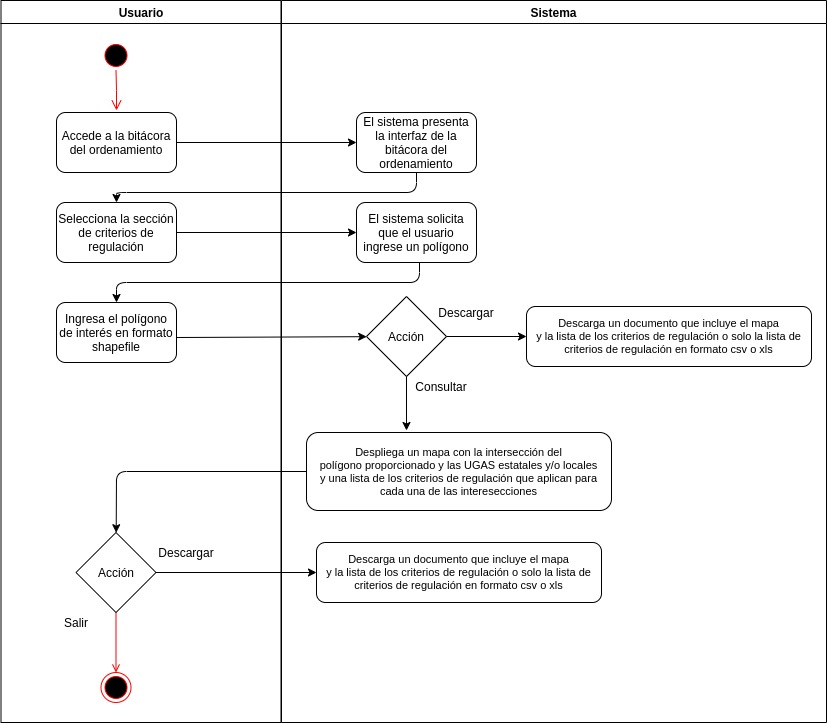
\includegraphics[width=0.8\textwidth, height=.37\textwidth]{images/diag_act_consultardescargar_critreg_poligono}
\end{figure}



%%%%%%%%%%%%%%% Actualizar-descargar recursos por UGAs
\pagebreak
\begin{figure}[h]
\centering
\caption{Diagrama de actividad \textbf{Actualizar-descargar recursos por UGAs}}\label{fig:priorReq}
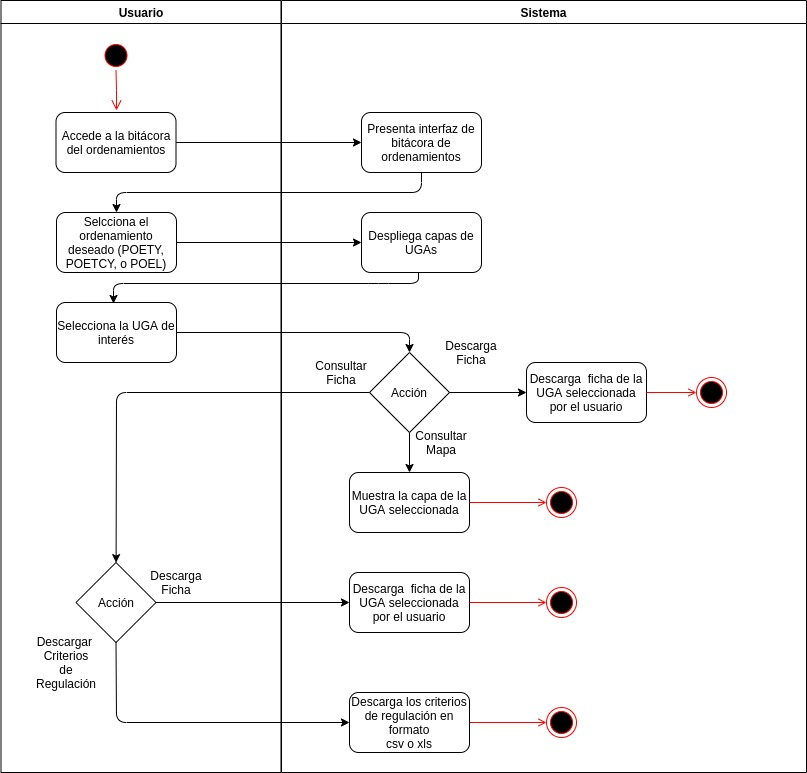
\includegraphics[width=0.8\textwidth, height=.5\textwidth]{images/diag_act_consultardescargar_UGAs}
\end{figure}

%%%%%%%%%%%%%%% Actualizar-descargar documentos relacionados con la formulación de ordenamiento
\pagebreak
\begin{figure}[h]
\centering
\caption{Diagrama de actividad \textbf{Actualizar-descargar documentos relacionados con la formulación de ordenamiento}}\label{fig:priorReq}
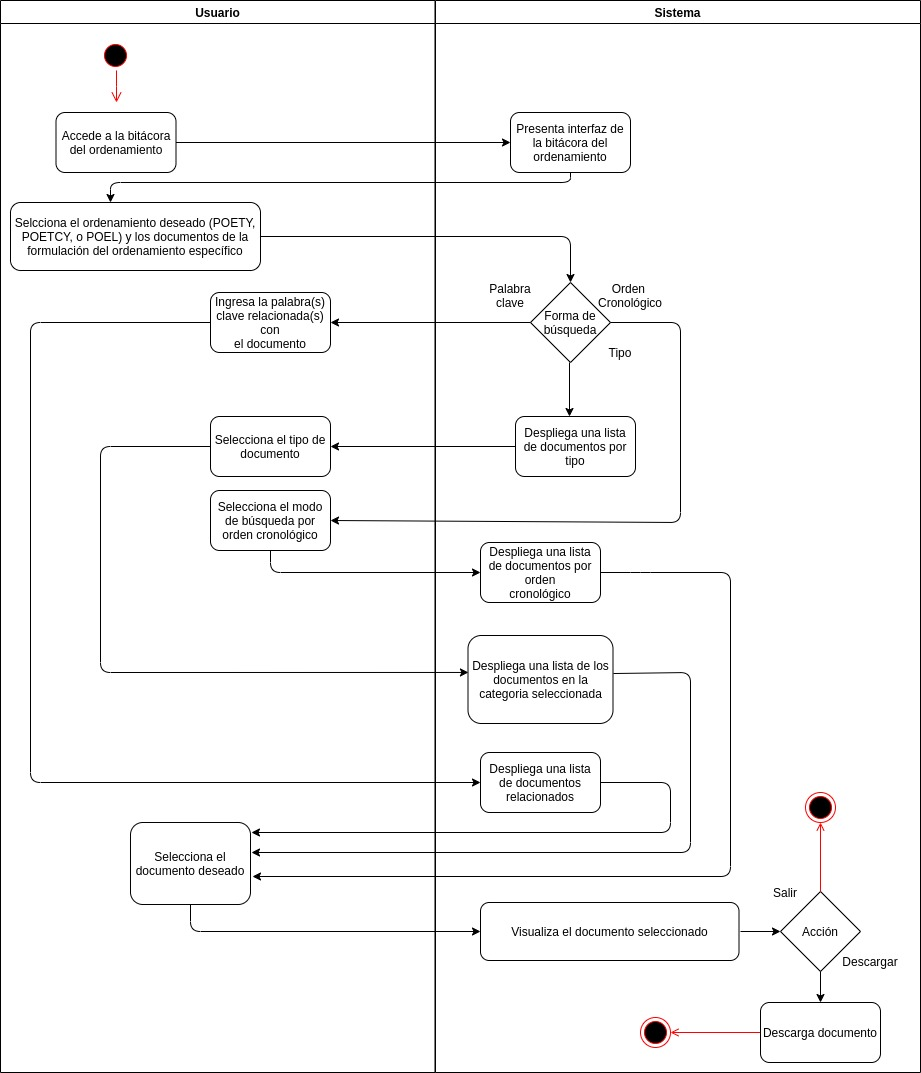
\includegraphics[width=0.8\textwidth, height=.6\textwidth]{images/diag_act_consultardescargar_doc_relac_form}
\end{figure}


%%%%%%%%%%%%%%% Actualizar-descargar capas de insumo para el ordenamiento
\pagebreak
\begin{figure}[h]
\centering
\caption{Diagrama de actividad \textbf{Actualizar-descargar capas de insumo para el ordenamiento}}\label{fig:priorReq}
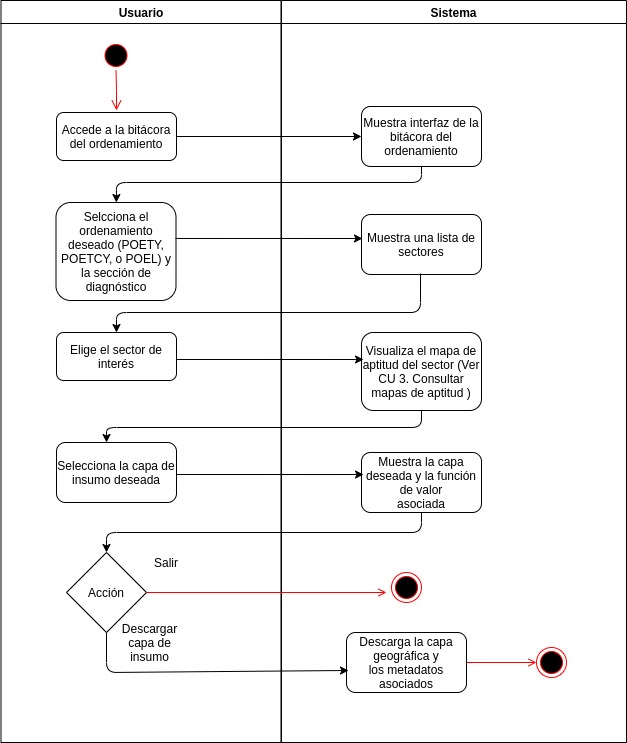
\includegraphics[width=0.8\textwidth, height=.5\textwidth]{images/dic_act_consultardescargar_capas_insumo_ordenamiento}
\end{figure}

\useportrait
\restoregeometry


%%%%%%%%%%%%%%%%%% Dar de Alta recurso 
\pagebreak
\begin{figure}[h]
\centering
\caption{Diagrama de actividad \textbf{Dar de Alta recurso}}
\label{fig:priorReq}
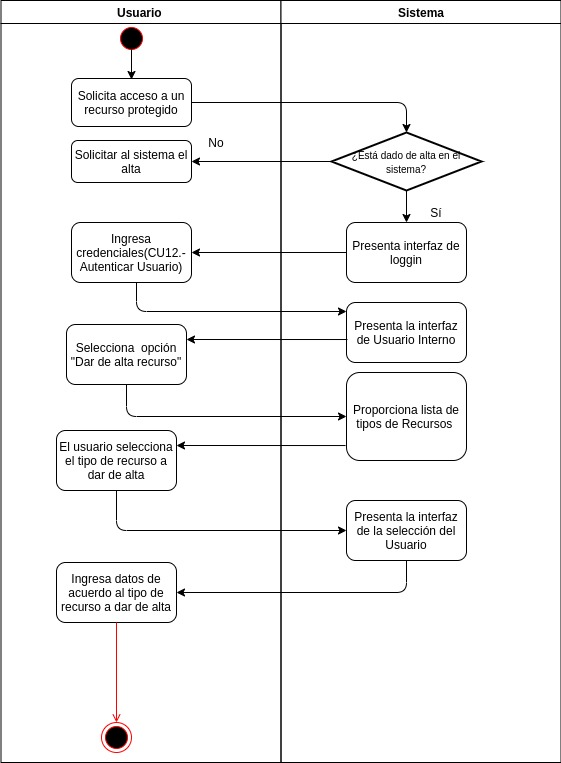
\includegraphics[width=1\textwidth, height=1.5\textwidth]{images/diag_act_alta_recurso}
\end{figure}

%%%%%%%%%%%%%%%%% Actualizar recurso
\pagebreak
\begin{figure}[h]
\centering
\caption{Diagrama de actividad \textbf{Actualizar recurso}}\label{fig:priorReq}
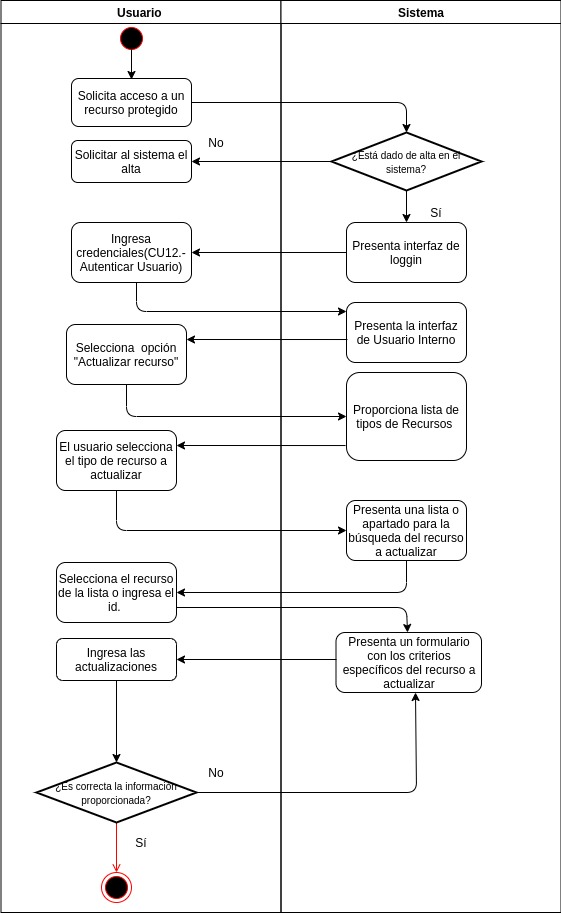
\includegraphics[width=1\textwidth, height=1.5\textwidth]{images/diag_act_actualizar_recurso}
\end{figure}

%%%%%%%%%%%%%%%% Borrar recurso
\pagebreak
\begin{figure}[h]
\centering
\caption{Diagrama de actividad \textbf{Borrar recurso}}\label{fig:priorReq}
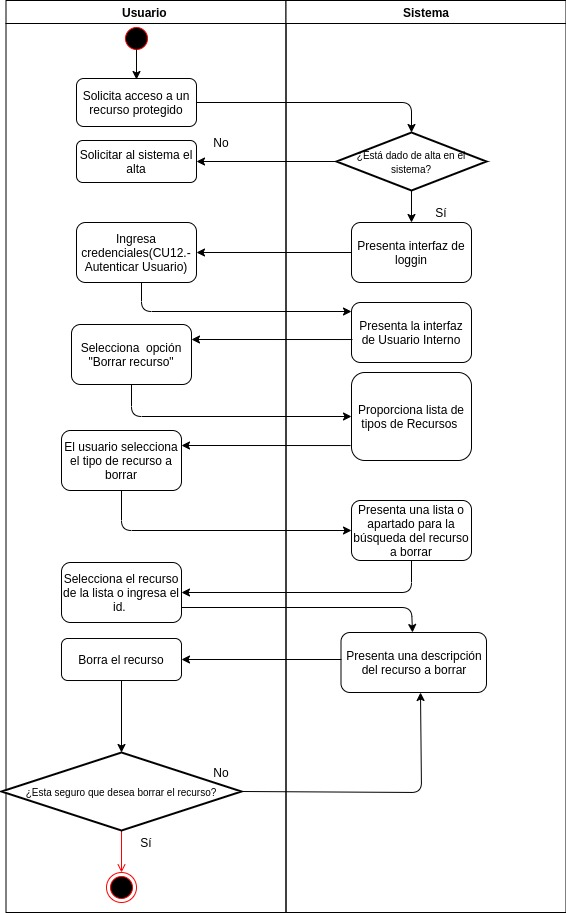
\includegraphics[width=1\textwidth, height=1.5\textwidth]{images/diag_act_borrar_recurso}
\end{figure}

%%%%%%%%%%%%%%%%%% Dar de Alta usuario 
\pagebreak
\begin{figure}[h]
\centering
\caption{Diagrama de actividad \textbf{Dar de Alta usuario}}
\label{fig:priorReq}
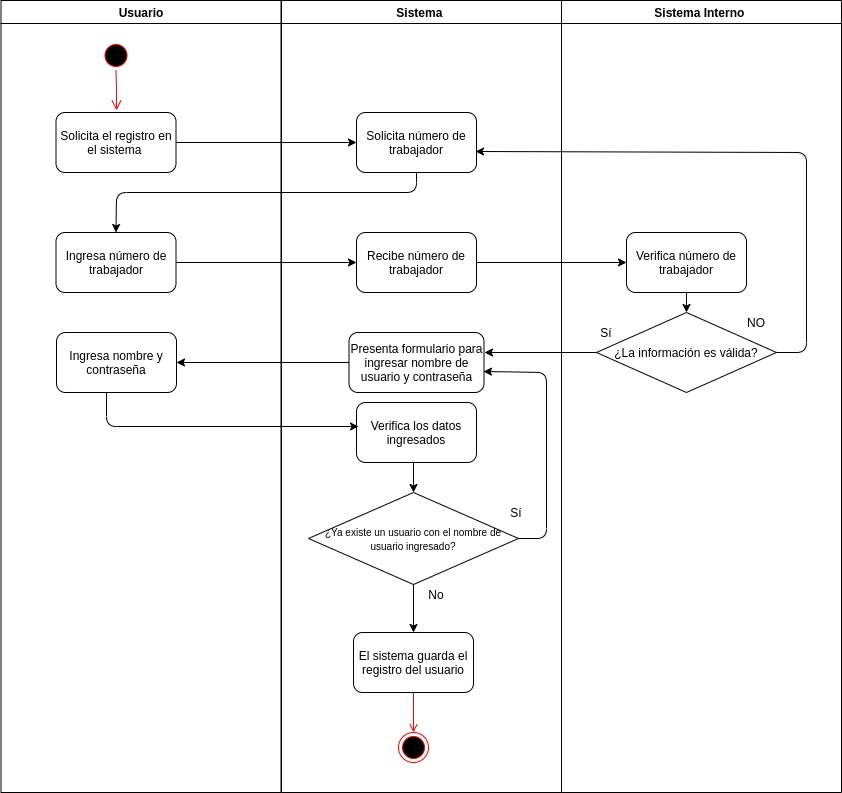
\includegraphics[width=1.2\textwidth, height=1.5\textwidth]{images/diag_act_alta_usuario}
\end{figure}

%%%%%%%%%%%%%%%%% Actualizar usuario
\pagebreak
\begin{figure}[h]
\centering
\caption{Diagrama de actividad \textbf{Actualizar usuario}}\label{fig:priorReq}
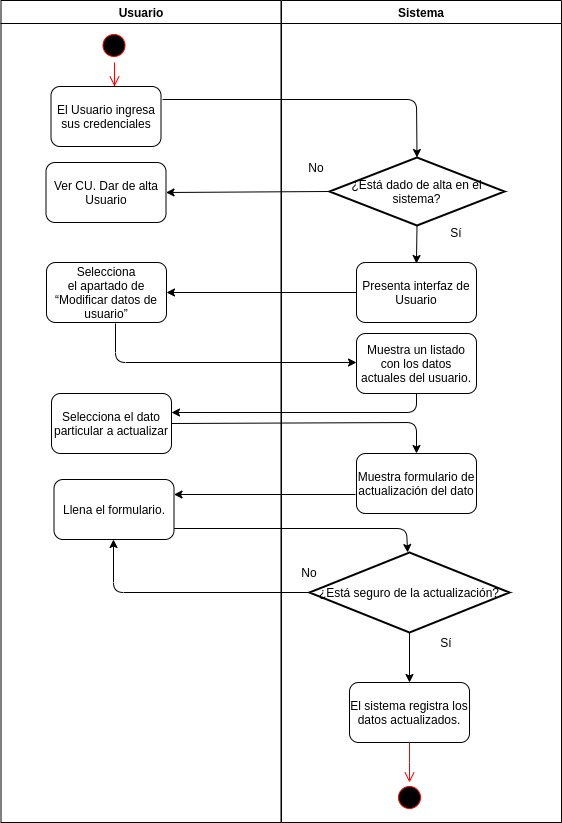
\includegraphics[width=1\textwidth, height=1.5\textwidth]{images/diag_act_actualizar_usuario}
\end{figure}

%%%%%%%%%%%%%%%% Borrar usuario
\pagebreak
\begin{figure}[h]
\centering
\caption{Diagrama de actividad \textbf{Borrar usuario}}\label{fig:priorReq}
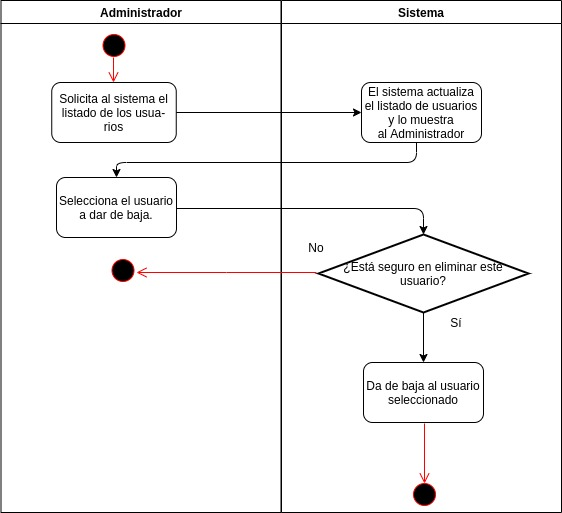
\includegraphics[width=1\textwidth, height=1.5\textwidth]{images/diag_act_borrar_usuario}
\end{figure}